    
    
    

    \hypertarget{Analysis III: Local and Fugal Analysis}{\chapter{Analysis III: Local and Fugal Analysis}\label{Analysis III: Local and Fugal Analysis}}


    \section{Fugal and Local Analysis
Objectives}\label{fugal-and-local-analysis-objectives}

    And finally, we have arrived at the final chapter of analysis for this
dissertation. It is this chapter that we finally will---more
importantly, can---move away from the more statistically centered
discourse and engage in discussion that is more rooted in traditional
music theory. Not only has the trajectory from general to local that has
been set in motion from the analysis from earlier chapters pointed us
towards the specifics of the fugal and thematic analyses of this
chapter, the statistical rigor of the earlier chapters have also granted
us with the freedom to engage in the more localized analysis in this
chapter, free from the fear of subconsciously cherry picking data, or
misinformed myopia.

In this final chapter, we will be focusing on examining intervals, but
this time on a fugal level, with the added parameters of subject and
motif. In doing so, we are shifting the attention away from contrapuntal
function, and directing the focus expressly towards the thematic and
expressive dimension of these intervals, and their role not so much as
functional building blocks, but as musical motifs and ideas. It is in
this chapter that we will embark upon our closest bid at significance,
not statistical significant, but artistic significance of temperament's
role in composition. We have seen statistical trends established in
earlier chapters linking temperament to interval usage; it is in this
chapter that we will go a step further and connect these trends to
specific fugal, thematic, and compositional elements that we know to be
significant in the fugal structure itself, attaching deeper musical
meaning and import to these intervals and the role they play in the
structural foundation and design of composition and key.

It is also in this final chapter that the genre of the fugue finally
comes into direct significance and analytical use. Musical structures
are deeply hierarchical, and one of the primary challenges of musical
analysis is to identify this hierarchical structure, and parse out
elements that are of musical or thematic significance from material that
serves more of a functional, supporting, or decorative role. In many
instances, this involves identifying the main musical forces, or
building blocks that comprise the compositional fabric. Compositionally,
there exist semantic building blocks, which can be see as intervals,
schemas, or stylistic elements that serve to fill out the musical
composition, but may not hold any significant further thematic
importance to the musical identity of the piece itself. Then there are
musical building blocks, which are comprised of (but not limited to)
recurring musical motifs, themes, and elements that define the
composition, in which its musical integrity hinges upon, and to which
alteration of these elements can potentially bring about a major
transformation---or complete dissolution---to the identity of a
piece and the musical ideas that it seeks to convey. If we can draw an
analogy of other compositional forms and their treatment of motivic
material to tenacious minds, then fugues are at the extreme end of
obsession, and Bach's fugues are beautifully neurotically so; he is a
master of the complete exploration of a subject through its endless
transformations and permutations, to achieve a transcendental level of
dual contrapuntal athleticism and sublime artistic expression. And in
analysis, this works very much to our advantage in accurately
identifying structure and importance.

For a fugue, its genre guarantees a higher degree of definition as to
what, and where, these musical building blocks are through its strict
adherence to the development of the subject material.
Essentially---and especially so in Bach---the subject,
countersubject, and its salient motifs are at the heart of what defines
and characterizes a fugal composition. They are not only the macro
building blocks of the fugue, but more importantly represent a microcosm
of the composition; if we can characterize the subject, we have in part
been able to characterize the entire fugue. And of these motivic
building blocks, the subject is especially so, as Ledbetter puts it,
"The inventio of a fugue is its subject, and this provides a microcosm
of the whole piece, not only in its technical ingredients but also in
its expressive nature" (Ledbetter, 2008, p.80). For this reason,
analyzing the fugal composition with attention to its subject is very
powerful, especially in discussing the musical integrity of a piece, but
it is still constraining our gaze to only a portion of the composition,
albeit arguably the most important portion. Thus, if we were to start
our analysis here, skipping the first two chapters, we could run the
possible risk of appearing incomplete or partisan; however, because we
have already established trends and correlations to exist consistently
and systematically outside of the fugal structure, this focus inward
upon fugal structure instead becomes the final logical step of analysis
to determine temperament's relationship to composition in a light that
focuses directly on musical and artistic importance, transcendent of
mere adherence to tradition and function, or to the service of other
more banal practicalities.

\subsection{Outline of Analysis}\label{outline-of-analysis}

Structurally, I will interleave fugal and local analysis in this chapter
in a discussion dictated by interval, breaking apart the analysis by
focusing on different intervals, and examining their usage within the
fugal and thematic structures (mainly the subject) of the compositions
that contain them. Within these sections, I will analyze in tandem how
temperament interacts with a composition's larger scale musical
structures such as structural architecture, approach to chromaticism,
and dissonance/consonance balance within these particular fugues, and
the keys that they are set in. Continuing the direction forged by the
last section in the previous chapter on scale degrees, this chapter will
largely focus upon intervals of the perfect and semitone class, as well
as analyzing fugues within the Pythagorean class keys.

Outline of analysis:

\begin{enumerate}
\def\labelenumi{\arabic{enumi}.}
\tightlist
\item
  Examine the usage of perfect intervals (fifths and fourths) as subject
  material, with the following focuses:

  \begin{enumerate}
  \def\labelenumii{\arabic{enumii}.}
  \tightlist
  \item
    Fifths and fourths as the opening interval of the fugue subject.
    Fugues analyzed:

    \begin{enumerate}
    \def\labelenumiii{\arabic{enumiii}.}
    \tightlist
    \item
      B-flat
    \item
      D-sharp minor
    \item
      C-sharp minor
    \end{enumerate}
  \item
    Fifths and fourths as general subject material.
  \end{enumerate}
\item
  Examine the usage of the simple semitone as subject material given
  duration in the following subsections:

  \begin{enumerate}
  \def\labelenumii{\arabic{enumii}.}
  \tightlist
  \item
    Opening semitone motifs longer than a quarter note (Pythagorean
    group). Fugues analyzed:

    \begin{enumerate}
    \def\labelenumiii{\arabic{enumiii}.}
    \tightlist
    \item
      F minor
    \item
      C-sharp minor
    \end{enumerate}
  \item
    Opening semitone motifs of a sixteenth note (meantone group). Fugues
    analyzed:

    \begin{enumerate}
    \def\labelenumiii{\arabic{enumiii}.}
    \tightlist
    \item
      C minor
    \item
      A minor
    \end{enumerate}
  \end{enumerate}
\item
  Examine the usage of the minor ninth as thematic material (subject and
  countersubject). The following breakdown:

  \begin{enumerate}
  \def\labelenumii{\arabic{enumii}.}
  \tightlist
  \item
    Ascending minor ninth as thematic material. Fugues analyzed:

    \begin{enumerate}
    \def\labelenumiii{\arabic{enumiii}.}
    \tightlist
    \item
      B-flat minor
    \end{enumerate}
  \item
    Descending minor ninth as thematic material. Fugues analyzed:

    \begin{enumerate}
    \def\labelenumiii{\arabic{enumiii}.}
    \tightlist
    \item
      B-flat minor
    \item
      F minor (countersubject)
    \end{enumerate}
  \end{enumerate}
\item
  Examine the relationship between special enharmonic and chromatic
  intervals against their more standard or diatonic counterparts to
  study how temperament can be used as a tool of harmonic reinforcement.
  Breakdown:

  \begin{enumerate}
  \def\labelenumii{\arabic{enumii}.}
  \tightlist
  \item
    Diminished fourth as subject material. Fugues analyzed:

    \begin{enumerate}
    \def\labelenumiii{\arabic{enumiii}.}
    \tightlist
    \item
      C-sharp minor
    \end{enumerate}
  \item
    Diminished seventh as subject material. Fugues analyzed:

    \begin{enumerate}
    \def\labelenumiii{\arabic{enumiii}.}
    \tightlist
    \item
      A minor
    \item
      D minor
    \item
      G minor
    \item
      B minor
    \end{enumerate}
  \item
    Chromatic perfect fourth as subject material. Fugues analyzed:

    \begin{enumerate}
    \def\labelenumiii{\arabic{enumiii}.}
    \tightlist
    \item
      F minor
    \end{enumerate}
  \end{enumerate}
\end{enumerate}

Before the concluding remarks of the chapter, I will offer a
comprehensive summary of the Pythagorean keys, and their fugal subjects,
main themes, and musical symbols that we have analyzed in this section,
as well as a summary of the conclusions that we have arrived at
regarding how these themes work together with the specific temperamental
structure of the keys of their respective fugues, ultimately giving rise
to the phenomenon of what musicians colloquially refer to as "key
characteristics". Through comparing the fugal subjects to their
respective key's temperamental scheme (scale degree charts), this
section will summarize how each of the fugue subjects for these
Pythagorean keys is in essence a microcosm and artistic representation
of the keys themselves, and that every one of these subjects cannot have
been realized in a key other than their own. The fugues---and their
key characteristics---that will be summarized in the chapter's
conclusion are as follows:

Summary of Pythagorean Keys:

\begin{enumerate}
\def\labelenumi{\arabic{enumi}.}
\tightlist
\item
  B-flat minor: summarize how the two important thematic intervals in
  its subject---the fifth and the minor ninth---work together to
  contribute to the very unusual color scheme and heightened
  expressivity of this fugue and its key.
\item
  D-sharp minor: summarize how the usage of fifths and fourths as
  prominent thematic material to demonstrate how these intervals play a
  central role to character and musical integrity of the piece, and
  contribute to the piece's character of solemnity and austerity.
\item
  C-sharp minor (with mention to companion modal Pythagorean minor key
  F-sharp minor): summarize how the tempering of c-sharp minor and its
  resulting smooth chromatic setting contributes to the structural arch
  of the piece through the specific construction of the first and final
  subjects.
\item
  F minor (with mention to companion boundary key B minor): summarize
  how the boundary nature of this key and its resulting accessibility to
  a wide contrast of interval types translates to musical contrast in an
  already dissonant fugue subject.
\end{enumerate}

The larger musical goals to be achieved in this final chapter are:

\begin{enumerate}
\def\labelenumi{\arabic{enumi}.}
\tightlist
\item
  Test the conclusions about temperament, key, and interval usage that
  have been suggested by previous chapters, and see if the predictions
  about the prevalence of usage of certain intervals given key and key
  group hold up on the fugal level.
\item
  Demonstrate that temperament's effect on key goes beyond mere
  compositional functionality, but has deep and direct implications on a
  key's specific characteristic and musical affect through its control
  on fugal, motivic, and thematic elements, that in turn exert effects
  on a composition's structural architecture, approach to chromaticism,
  and dissonance/consonance profile.
\item
  Demonstrate that keys are not interchangeable, both within and without
  key groups, and that certain important thematic and structural
  elements constructed in a specific keys will fall apart and become
  rendered ineffective post-modulation.
\end{enumerate}

The culmination of these goals wrap around to affirm the main objective
of this thesis: to state that there is indeed robust and prolific
evidence to believe that Bach approached composition with temperament in
mind, and thoughtfully selected subjects, motifs, and themes for certain
pieces based on key and their attributes as dictated by the
well-tempered tuning system. Moreover, the analysis in this chapter on
temperament and its relationship to interval choice within fugal
subjects, themes, and motivic material demonstrates that these
compositional decisions go beyond the historical and functional realm,
but are more importantly decisions moved by musical and artistic
motivations. Ultimately, temperament's involvement on these various
levels of composition illustrate a dynamic, complex, and intimate
relationship between it and a composition's functional, historical, and
musical integrity, and is far from being a mere technical artifact and
should not be dismissed as such.

    \section{Perfect Intervals (Fifths and Fourths) as Subject
Matter}\label{perfect-intervals-fifths-and-fourths-as-subject-matter}

We have already established in earlier chapters a strong connection
between the Pythagorean class keys---and even more so, the exemplar
keys of b-flat and d-sharp---and pure intervals (especially the
fifth), namely that Pythagorean keys utilize these intervals more
frequently, specifically the pure versions. This section will now add
the extra parameter of searching solely within fifths found in the
subject material of fugues, to look specifically at how the perfect
fifth is prominently featured as purposeful, motivic material that is
integral to a piece's thematic import and coherence.

It is very true that the fifth (along with the other intervals we have
been examining, the third and the semitone), are staple intervals widely
utilized within the general western tonal language, which include
species counterpoint and the contrapuntal style of Bach. As a result,
many statements of these intervals that we have encountered in the
Well-Tempered Clavier may have little to do with motivic salience, but
rather just play a functional role as dictated by the contrapuntal
design and rules governing species counterpoint and voice leading. These
functional instances of intervals are far from unimportant, but
constraining our gaze to only fifths within fugal subjects will allow us
to focus upon the relationship between key and the usage of fifth as
purposeful motivic material, instead of mere contrapuntal function.

Motivically, the fifth and fourth, especially in an open setting (i.e.
not immediately filled in or arpeggiated by a third) is a rather special
interval in the context of the new well-tempered system, as it hearkens
back to a more archaic sound and harmony that had belonged to the bygone
Pythagorean era of tuning, which had been phased out during the
Rennaissance in favor of meantone tuning. With the resurgence of the
purity of these perfect intervals with the advent of well-temperament
came the reintroduction to the resonance and openness of quartal
harmony, a sound that had been sacrificed in favor of the more
mellifluous and colorful tones of tertiary harmony. Indeed, when
presented in their pure, untempered form, there is an openness and
austerity to the perfect class intervals (due to their lower position on
the harmonic series) that is deeply grounding and powerful, a certain
primal nature of a harmony that was favored for centuries as a
cornerstone of the first and longest standing tuning system in the
western tonal tradition.

Musically speaking, the openness and lack of modal color gives these
intervals heightened power and resonance in their pure configurations,
and their low position on the harmonic series adds a certain chameleon
quality: under certain settings, these intervals can be incredibly
calming and meditative, but in a different context, severe and eerie.
Indeed, composers and musicians from both past and modern times have
utilized these intervals for precisely these varying musical effects
(think tanpura drones in Indian music, power chords in the blues and
rock genres, and those powerful, austere open fifth cadences brilliantly
employed in Mozart's Requiem). Following this line of thinking, it is
logical that Bach's employment of these perfect intervals as thematic
material would also stem from the same sensitivity towards the
intervals' resonant power, which would in turn inform the character and
design of a fugue's subject that is constructed upon them. Furthermore,
we should expect to see a predilection towards the pure versions of
these intervals for these thematic statements, as well as setting these
compositions built upon perfect intervals in keys that would most
support their interval purity.

Before we get into fully analyzing these perfect intervals in the
context of theme, motif, and fugal subject, let us recap a bit by first
reviewing a chart of all horizontal fifths, both within and without the
subject, of all the minor fugues for overview:



    \begin{center}
    \adjustimage{max size={0.6\linewidth}{0.9\paperheight}}{analysis_3_files/analysis_3_7_0.png}
    \end{center}
    
    The result from this chart is in line with what we would expect given
the analysis from previous chapters; theoretically, pure fifths
outnumber tempered fifths 2 to 1, so in a completely fair split, our
expected values for this chart should be 33.33\% tempered intervals to
66.6\% pure intervals. However, the numbers are skewed towards the pure
intervals, which is again expected, given what we have already
demonstrated in earlier chapters of Bach favoring the usage of the fifth
in Pythagorean keys, which on a whole are designed to favor pure fifths
over tempered fifths. With these values in mind, let us now add the
parameter of subject onto this distribution; that is to say, let us look
at the distribution of fifths across all minor fugue subjects:




\begin{figure}[H]
    \begin{center}
    \adjustimage{max size={0.6\linewidth}{0.9\paperheight}}{analysis_3_files/analysis_3_10_0.png}
    \caption{Fifths in All Minor Fugue Subjects}
    \end{center}
\end{figure}
    
    Immediately, we can observe a sizable jump for the pure intervals, as
its value increases almost by 10\%. The values of this graph indicates
that more than 80\% of subject fifths are pure, as opposed to 70\% of
fifths being pure when we consider subject and nonsubject material
together. This increase is indicative that the purity of this interval
does not just pertain to a conscious choice in regards to function, but
even more so in consideration to a musical decision involving motif and
thematic material.

Furthermore, in line with what we have observed of the connection
between fifths and Pythagorean keys, the following (first) chart
superimposes upon the previous chart of fifths in minor fugue subjects
(in blue) the chart of fifths in only the Pythagorean fugues (in red).
From this chart, we observe that an overwhelming majority of these
subject fifths occur in Pythagorean keys, specifically, 75\% of fifths,
of which 98\% of these Pythagorean subject fifths are pure
(73.08/(1.47+73.08)). The second chart look at only Pythagorean fugues,
comparing all fifths in the general (subject and non-subject material)
composition in blue, and the subject material fifths (in red). The
reason for this comparison is to put the percentage of pure fifths in
the fugue subjects (98\%) in context. As we can observe from the blue
bars (all fifths in Pythagorean fugues regardless of subjects), pure
fifths constitute around 91\% of all fifths, however, when we restrict
this search to only subject fifths, the value increases to 98\%.




\begin{figure}[H]
    \begin{center}
    \adjustimage{max size={0.6\linewidth}{0.9\paperheight}}{analysis_3_files/analysis_3_13_0.png}
    \caption{All fugue fifths comparison chart}
    \end{center}
\end{figure}
    



\begin{figure}[H]
    \begin{center}
    \adjustimage{max size={0.6\linewidth}{0.9\paperheight}}{analysis_3_files/analysis_3_15_0.png}
    \caption{Pythagorean fugue fifths comparison chart}
    \end{center}
\end{figure}
    

    From the progression across these initial charts of fifths, we can
already observe that pure fifths are selected for thematic and motivic
use. Specifically, and fugally, there is an increase of usage of the
fifth in the subject in keys and key groups that contain the highest
amount of pure perfect intervals: the Pythagorean class keys. A summary
integrating the conclusions drawn from the above charts are as follows,
in which we can see how pure fifths are increasingly used as place on
additional parameters to control for subject and key:

\begin{itemize}
\tightlist
\item
  Without controlling for subject, pure fifths constitute around 71\% of
  fifths in the general compositional material in the minor fugues. This
  5\% above the expected value of 66\%, based purely on the number of
  available pure fifths to tempered fifths within Werckmeister III.
\item
  When restricting the material to looking only within fugal subjects,
  we see an increase of pure fifths to constitute 82\% of all fifths, an
  increase of 9\%.
\item
  Of all the fifths (pure and tempered) found in fugal subjects, 75\% of
  these fifths belong to Pythagorean class keys.
\item
  Of these Pythagorean fugue fifths, 98\% of the subject fifths are
  pure, as opposed to the 91\% of pure fifths when looking at general
  compositional material in these keys.
\end{itemize}

    \subsection{Perfect Intervals as the Opening Interval to a Subject
Statement (B-flat, D-sharp, C-sharp
minor)}\label{perfect-intervals-as-the-opening-interval-to-a-subject-statement-b-flat-d-sharp-c-sharp-minor}

\subsubsection{First Subject Opening: B-flat and D-sharp Minor
Fugues}\label{first-subject-opening-b-flat-and-d-sharp-minor-fugues}

Having now established a general positive relationship between
fifths---specifically pure fifths---and their usage as subject
material, we will now turn our attention to more detailed analyses on
how these fifths are used within these subjects, and how the specific
tempering and key settings work together with the subject material to
contribute to the resulting musical structures and general character of
these compositions.

If the subject is motivically the most prominent thematic force within
the fugal form, the opening interval of the subject is even more so, as
it is not only our first encounter with the subject, but with the entire
composition. The following Python search extracts the fugues from WTC
I---if any---that contain either a fifth or fourth as its
opening interval; we will also display the subjects from the fugues
detected:

    \begin{Verbatim}[commandchars=\\\{\}]
{\color{incolor}In [{\color{incolor}5}]:} \PY{n}{d}\PY{o}{=}\PY{n}{m\PYZus{}hz\PYZus{}concat\PYZus{}wk}
        \PY{n}{df}\PY{o}{=}\PY{n}{d}\PY{p}{[}\PY{p}{(}\PY{n}{d}\PY{p}{[}\PY{l+s+s1}{\PYZsq{}}\PY{l+s+s1}{int class}\PY{l+s+s1}{\PYZsq{}}\PY{p}{]}\PY{o}{==}\PY{l+m+mi}{5}\PY{p}{)}\PY{o}{\PYZam{}}\PY{p}{(}\PY{n}{d}\PY{p}{[}\PY{l+s+s1}{\PYZsq{}}\PY{l+s+s1}{subject 1}\PY{l+s+s1}{\PYZsq{}}\PY{p}{]}\PY{o}{==}\PY{l+s+s1}{\PYZsq{}}\PY{l+s+s1}{True}\PY{l+s+s1}{\PYZsq{}}\PY{p}{)}\PY{o}{\PYZam{}}\PY{p}{(}\PY{n}{d}\PY{p}{[}\PY{l+s+s1}{\PYZsq{}}\PY{l+s+s1}{subject offset}\PY{l+s+s1}{\PYZsq{}}\PY{p}{]}\PY{o}{==}\PY{l+m+mi}{0}\PY{p}{)}\PY{p}{]}
        \PY{n}{df}\PY{o}{.}\PY{n}{index}\PY{o}{.}\PY{n}{unique}\PY{p}{(}\PY{n}{level}\PY{o}{=}\PY{l+m+mi}{0}\PY{p}{)}
\end{Verbatim}
\begin{Verbatim}[commandchars=\\\{\}]
{\color{outcolor}Out[{\color{outcolor}5}]:} Index(['dsh\_1', 'bfl\_1'], dtype='object')
\end{Verbatim}


\begin{Example}[H]
    \begin{center}
    \adjustimage{max size={0.9\linewidth}{0.9\paperheight}}{analysis_3_files/analysis_3_21_0.png}
    \caption{ D-sharp minor fugue subject (mm. 1-3). }
    \end{center}
\end{Example}
    


\begin{Example}[H]
    \begin{center}
    \adjustimage{max size={0.9\linewidth}{0.9\paperheight}}{analysis_3_files/analysis_3_23_0.png}
    \caption{ B-flat minor fugue subject (mm. 1-4). }
    \end{center}
\end{Example}
    
    The two fugues yielded by this inquiry are none other than the two
exemplar Pythagorean fugues, b-flat and d-sharp minor. This is
completely in line with the results and expectations from our analyses
in the previous chapters, which show the strongest links between pure
fifths and these two keys. The fact that Bach chooses these two, and
only these two, fugues to contain this very interval as their subjects'
opening interval is an indicative gesture of a purposeful desire to
feature this interval in a musically and thematically prominent way in
these specific keys.

In line with the temperamental expectation of these two keys, not only
do both fugues contain the pure version of the perfect interval at this
opening position, but almost every instance of the subject fifth/fourth
is pure. The two charts below corroborate this information on the purity
of the opening interval to the first subject statement for both the
b-flat minor and d-sharp minor fugues, with the d-sharp minor chart
containing the additional two statements of the fifth within its
subject. The graphs immediately following contain the distribution of
every occurrence of subject fifths/fourths of each fugue as a function
of interval purity.

For each key, two slightly different versions of the subject graphs are
provided, in accordance to the way these thematic fifths are utilized in
their respective compositions, which I will unpack in more detail after
the presentation of the graphs. For d-sharp minor, the graph on the left
contains only opening subject fifths/fourths, the graph on the right
includes all subject perfect intervals. For the b-flat minor graph, the
leftmost graph contains only subject fifths/fourths in complete subject
statements, and the rightmost graph contain all subject/thematic
fifths/fourths, which also include partial subject statements and the
motivic derivations of this descending subject fifth/fourth. The reasons
for these two graphs for each piece, especially the two b-flat minor
graphs, will become more apparent in the analysis offered below.

What can be corroborated immediately through the graphs though is the
vast prevalence of pure fifths in both the d-sharp and b-flat minor
fugues. For the d-sharp minor fugue, a dramatic 29 out of 31 opening
perfect intervals are pure, when taking in account all subject fifths,
92 out of 100 intervals are pure. For b-flat minor, the difference is
even greater; all 21 full subject fifths/fourths are pure, for thematic
fifths, only one fifth is tempered out of the 29 total.

\begin{Verbatim}[commandchars=\\\{\}]
      file  cents from just  ic nb sc directed name subject  subject offset  \textbackslash{}
484  dsh\_1                0       0.0            P5    True             0.0   
491  dsh\_1                0       0.0           P-5    True             5.0   
492  dsh\_1                0       5.0            P4    True             6.0   

     measure  
484        1  
491        2  
492        2  
\end{Verbatim}
\begin{Verbatim}[commandchars=\\\{\}]
    file  cents from just  ic nb sc directed name subject  subject offset  \textbackslash{}
0  bfl\_1                0       0.0           P-4    True             0.0   

   measure  
0        1  
\end{Verbatim}

    \begin{center}
    \adjustimage{max size={0.9\linewidth}{0.9\paperheight}}{analysis_3_files/analysis_3_27_0.png}
    \end{center}
    

    \begin{center}
    \adjustimage{max size={0.9\linewidth}{0.9\paperheight}}{analysis_3_files/analysis_3_28_0.png}
    \end{center}
    
    Indeed, to say that these two fugues utilize the fifth as important
thematic material is an understatement, as both the vertical and
horizontal structures of the two fugues are entirely constructed upon
the theme of the fifth, and the exhaustive exploration of its sonic
possibilities. Nowhere else in the Well-Tempered Clavier does Bach even
come close to this level of dedication to this particular
interval---perhaps any other singular interval, for that
matter---as thematic material; in some way, the interval itself is
almost featured more prominently than the entire rest of the subject
that adorns it. Additionally, both pieces are obsessive about the
subject itself in both its repetition as well as contrapuntal
development, which are central components to the resulting structure of
both fugues.

Interestingly enough, both subjects share essentially the same opening
portion in both pitch and rhythm, with the exception of b-flat minor
being an augmentation of the quicker note values of d-sharp minor, with
a rest after its opening statement of the fifth instead of holding the
second note, and instead of the interval of an ascending fifth that we
find in the d-sharp minor fugue, the fugue in b-flat opens with a
descending fourth, the fifth inverted. Because the opening interval is a
perfect interval, the answer is tonal, in this case, allowing for the
presentation of both the fifth and the fourth as subject material as the
piece unfolds. Both subjects are also slow, allowing for a greater
degree of acoustical resonance, and in both cases, all of the perfect
intervals within the subject are assigned note values that are twice as
long as the rest of the subject, calling our attention to these
intervals as well as accentuating the resonant potential of these
particular intervals.

Furthermore, both subjects contain additional elements to call special
attention to the motif of the perfect interval, and its resonant
character, even beyond having the interval as their opening statements.
For the b-flat minor fugue, the half notes assigned to the opening
fourth, set in cut time, and followed immediately by a quarter note rest
not only gives this opening interval a tremendous amount of gravity and
inertia, but essentially sets it apart from the rest of the subject,
almost dividing the subject into two portions (Bach does this quite
often in terms of dividing longer subjects into shorter motivic sections
that can be individually developed). Indeed, this opening subject motif
of the descending fourth in half notes will often appear on its own
outside of the subject throughout the rest of the piece. Although there
are not as many full subject statement as the d-sharp minor fugue (22 as
opposed to an astounding 36), these ubiquitous statements of the opening
motif allow this subject fifth (and the presence of the subject) to
permeate throughout the structure of the piece, even without the entire
subject needing to be stated.

Below is an example of how this statements of the subject (tonal answer)
in stretto in the b-flat minor fugue (mm. 50-54), along with clever
usage of the fifth motif as a connector collectively creates a string of
cascading falling fifths. The soprano starts the cascade on the high F
in the first measure, followed immediately by the alto voice in stretto
on the second beat of that measure, which pitches are echoed in the bass
voice in the next measure, continuing the falling fifths down to a-flat,
to which the tenor II comes in with the subject again in the next
measure, all in all creating a seamless wall of resonance in which the
second portion of the subject floats upon. Note also the eliding notes
created by the stretto; a modern piano would unfortunately preclude the
doubled pitch, however, a double manual instrument of Bach's day would
have easily presented the simultaneous pitches, further adding to the
thickness of the sonic texture, and increasing the resonance of these
fifths. In fact, doubled notes are a very common feature of this fugue,
as the five voices command a very thick and compact sonic texture, and
on an instrument with multiple manuals, all these doubled (or tripled)
notes would have contributed even more to the thickness of the texture,
and overall acoustical resonance of the piece.



\begin{Example}[H]
    \begin{center}
    \adjustimage{max size={0.9\linewidth}{0.9\paperheight}}{analysis_3_files/analysis_3_31_0.png}
    \caption{ Falling fifths in b-flat minor fugue (mm. 50-54). }
    \end{center}
\end{Example}
    
    For the d-sharp minor fugue, the subject highlights the fifth in a
slightly different fashion, mainly through repetition within the
subject, and thorough subject transformation and development that
dictates the structure of the piece. Within the subject itself, the
opening thematic perfect interval motif is essentially featured twice in
the same rhythmic scheme, first on the interval of a fifth, and a second
time on the interval of a fourth. Additionally, a descending fifth, also
in quarter notes, joins the two thematic motifs, adding yet another
perfect interval to the subject statement. This subject is then
extensively developed through means of extreme stretto (more on this
device in the following paragraph), augmentation, and inversion, the
former two elements bolstering the resonance of the fifths through
clever contrapuntal arrangement into vertical configuration, and
lengthening of duration, and the latter element of inversion playing a
major force in the compositional structure of the fugue, as the subject
inverso is given its own development and tantamount attention to the
subject recto. The subject inverso also allows for even more permutation
of the thematic perfect interval, in this case, instances of descending
fifths, which Bach uses for its own distinct coloristic effect. An
example of this (shown directly below) can be seen at the beginning of
the stretto inverso exposition (m.44), which begins with knelling fifths
stated in the bass, and further modified to contain two iterations of
the fifth, as opposed to a fifth and a fourth. These knelling fifths are
further repeated in stretto by the soprano voice a beat after,
reminiscent of an echo-like effect that would result from a knelling
bell. Thus, even though D-sharp minor has a more flowing tempo and
lingers less on any specific instance of the thematic fifth, the
repetition of the interval within the subject, as well as dedication to
its extreme development results in more iterations of the subject fifth
and fourth throughout the course of the fugue.



\begin{Example}[H]
    \begin{center}
    \adjustimage{max size={0.9\linewidth}{0.9\paperheight}}{analysis_3_files/analysis_3_34_0.png}
    \caption{ Knelling fifths in d-sharp minor fugue (mm. 44-47). }
    \end{center}
\end{Example}
    
    One other crucial feature that both these fugues have in common is the
compositional device of stretto, which both compositions employ to an
extreme degree, and which is central to both fugues' resulting vertical
structures, as well as their formal organizational structure and
resulting architecture. Essentially, stretto plays a major component to
the formal design of both fugues, both of which are exposition fugues,
and to which each subsequent subject exposition gradually introduces an
increasingly intense and intricate involvement of stretto. For the
d-sharp minor fugue, this culminates in a masterful stretto of the three
voices, each varied under different levels of augmentation (bass in
original form, mezzo in partial augmentation, and soprano in full
augmentation), bearing resemblance to the contrapuntal technique of the
mensuration canon of the medieval and Renaissance periods.



\begin{Example}[H]
    \begin{center}
    \adjustimage{max size={0.9\linewidth}{0.9\paperheight}}{analysis_3_files/analysis_3_37_0.png}
    \caption{ Stretto and augmentation in d-sharp minor fugue (mm. 77-80). }
    \end{center}
\end{Example}
    
    In the case of the b-flat minor fugue, Bach concludes the piece with a
brilliant five-part \emph{stretto maestraele} (meaning that all subjects
are presented in their complete material) at the half measure, starting
in order of vocal tessitura from the soprano all the way down to the
bass (shown in the first four bars of the excerpt below). This chain of
falling fifths mirrors the order of the vocal presentation from the
first exposition, providing a sense of formal return and closure, but it
is not quite a return to the same forlorn landscape that we started on
at the beginning of this journey. The final presentation of the subjects
in stretto transforms the subject into one of heightened splendor and
grandeur, its once stark open fifth and pleading minor ninth filled out
in brilliant doublings and full five-voice chorus of harmony. Indeed,
this final \emph{streto maestraele} serves as not only an inevitable
conclusion to the overall sonic structure of a piece that features
through gradual terracing the building up of texture and sonority
through the means of stretto, but also presents a sort of microcosmic
representation and summary of this structure.

We would expect this incredible demonstration of contrapuntal mastery of
the \emph{stretto maestraele} to be the final word on the theme of the
falling perfect intervals, but Bach, in a very Bachian manner, has a
final surprise in store at the very conclusion of the fugue (also
observable in the end excerpt provided below). At the unexpected event
of the C major chord two measures from the end at bar 73 (harmonically
unexpected as the tonic 6/4 chord in the previous measure implies the
initiation of the cadential 6/4, which would lead us to expect an
immediate presentation of a V chord in the following bar, not a V/V C
Major chord to delay the dominant), Bach initiates a final series of
falling fifths, this time tracing through the circle of fifths in
retrograde from G all the way to the final arrival of the B-flat tonic
at the very conclusion of the piece. As the \emph{stretto maestraele}
provided a fitting conclusion to the subject and the fifths therein,
this final iteration of falling, retrogade circle of fifths also
provides a conclusion to the theme of free falling fifths that were so
motivically integral to the structure of the fugue, and in doing so
solidifies without a doubt the central importance of the perfect
interval in the thematic and artistic integrity of this fugue.

Finally, this closing cadence provides a beautiful final gestural and
harmonic closure of the motifs within the subject itself. Without
calling a formal statement of the subject, Bach nonetheless evokes the
thematic material of the subject a final time: the perfect interval
through the motion of the falling, motivic fifths, and the minor ninth
(which we will analyze in depth in the next section involving semitones)
through the jarring dissonance presented by the harmonic minor ninth on
the V/V C major chord in bar 72. This time, however, he finally resolves
the implied query and tension posed initially by both these subject
intervals, resolving the lingering opening fourth statement and its
pause on the dominant down to the tonic, and settling the descending
line proceeding the minor ninth down to the tonic as well, this time
finally resolving its downward motion, and bringing to rest its ethereal
meandering.



\begin{Example}[H]
    \begin{center}
    \adjustimage{max size={0.9\linewidth}{0.9\paperheight}}{analysis_3_files/analysis_3_40_0.png}
    \caption{ Stretto maestraele in b-flat minor fugue (mm. 67-75). }
    \end{center}
\end{Example}
    
    A final word on vertical texture as informed by stretto: both fugues use
stretto in conjunction with the thematic fifth to create a prominent
presence of harmonic fifths and fourths on the vertical domain; this not
only increases the level of sonority and resonance on a purely acoustic
level, but is also a stylistic nod on the compositional level to the
Pythagorean tradition of quartal harmony that favored these intervals
over the third as their primary building blocks. The effect of these
elements of quartal-like harmony and the resulting resonance manifests
itself artistically in slightly different ways for each fugue, mostly
due to the vocal forces available. For the 3-voice d-sharp minor fugue,
the sonic landscape is thinner, lending the perfect intervals to a more
forlorn quality of sound and contrapuntal arrangements that create
instances of severity and austerity of sound. An illustration of this
can be seen in the beginning of the stretto recto and inverso exposition
(m. 52): the ascending fourth gesture of a\#-d\# is iterated in each
voice, presented sequentially in stretto staggered by a quarter note,
yielding a sequence of knelling simple vertical open fifths. The
resulting harmony of these vertical fifths in isolation is rather eerie,
as the ear accustomed to the gentle complexities of tertiary harmony is
not used to hearing bare fifths unadorned in this fashion, a starkness
that hearkens back to medieval style polyphony and harmonic texture.



\begin{Example}[H]
    \begin{center}
    \adjustimage{max size={0.9\linewidth}{0.9\paperheight}}{analysis_3_files/analysis_3_43_0.png}
    \caption{ Vertical quartal harmony in d-sharp minor fugue (mm. 52-53). }
    \end{center}
\end{Example}
    
    For the thicker, impressive vocal forces of the 5-voice b-flat minor
fugue, these fifths in conjunction to the rich vocal texture allow for
the maximization of a sonorous, chorale-like setting (the grand
\emph{stretto maestraele} being a prime example of this). Like in the
d-sharp minor fugue, Bach strategically uses these strettos to further
set up harmonic and contrapuntal moments that are more reminiscent of
the older, Gothic style polyphony that utilized Pythagorean tuning and
these pure perfect intervals. In the following example (shown below), we
observe that the fourth subject exposition features a simultaneous
subject entry (immediate stretto), its onset coinciding with the arrival
of the tonic chord from the conclusion of the previous exposition,
creating an elided cadence (m. 55 in the original score, second measure
shown in excerpt). The way that the elided tonic chord is voiced
emphasizes heavily the interval of the fourth and fifth, and its
interaction with the tonic, creating an 8/5 trine in the highest three
voices (both an elevated and essential harmonic force in 13th century
polyphony), reinforced with a tripled tonic in the bass, with only a
passing quarter note assigned to the third. This trine created by the
upper three voices, a three-voice harmony comprised of a lower fifth and
upper fourth, outlining an octave, was a staple harmony of the 13th
century polyphonic setting, as it was viewed as complete, perfect
harmony in their Pythagorean tuning system, which ensured pure
sonorities on all intervallic combinations within the chord. It was the
most stable configuration of an interval in this system, and thus
regarded as the ideal goal in a cadential setting. This focus on quartal
construction here is further bolstered with the second interval of a
perfect fourth created by the subject, and the trine and fourth further
strengthened and placed in a position of heightened emphasis by this
presence of the double subject in stretto.



\begin{Example}[H]
    \begin{center}
    \adjustimage{max size={0.9\linewidth}{0.9\paperheight}}{analysis_3_files/analysis_3_46_0.png}
    \caption{ Cadential trine in b-flat minor fugue (mm. 54-56). }
    \end{center}
\end{Example}
    
    Through this examination of Bach's usage of the fifth and fourth in a
thematic setting within the subjects of these two fugues, it is evident
that the perfect interval is a central building block to not only the
thematic and formal structure to both compositions, but also to the
acoustical resonant property to create a sense of sonic space and
solemnity of character.

\subsubsection{Other Subjects Opening: C\# Minor
Fugue}\label{other-subjects-opening-c-minor-fugue}

We will now ask the question again, but this time include second and
third subject statements into the mix. Although an opening interval of a
second or third subject no longer serves as the opening interval to the
composition itself, it nonetheless still holds a great deal of thematic
importance:

    \begin{Verbatim}[commandchars=\\\{\}]
{\color{incolor}In [{\color{incolor}4}]:} \PY{n}{d}\PY{o}{=}\PY{n}{m\PYZus{}hz\PYZus{}concat\PYZus{}wk}
        \PY{n}{df}\PY{o}{=}\PY{n}{d}\PY{p}{[}\PY{p}{(}\PY{n}{d}\PY{p}{[}\PY{l+s+s1}{\PYZsq{}}\PY{l+s+s1}{int class}\PY{l+s+s1}{\PYZsq{}}\PY{p}{]}\PY{o}{==}\PY{l+m+mi}{5}\PY{p}{)}\PY{o}{\PYZam{}}\PY{p}{(}\PY{n}{d}\PY{p}{[}\PY{l+s+s1}{\PYZsq{}}\PY{l+s+s1}{subject}\PY{l+s+s1}{\PYZsq{}}\PY{p}{]}\PY{o}{==}\PY{l+s+s1}{\PYZsq{}}\PY{l+s+s1}{True}\PY{l+s+s1}{\PYZsq{}}\PY{p}{)}\PY{o}{\PYZam{}}\PY{p}{(}\PY{n}{d}\PY{p}{[}\PY{l+s+s1}{\PYZsq{}}\PY{l+s+s1}{subject offset}\PY{l+s+s1}{\PYZsq{}}\PY{p}{]}\PY{o}{==}\PY{l+m+mi}{0}\PY{p}{)}\PY{p}{]}
        \PY{n}{df}\PY{o}{.}\PY{n}{index}\PY{o}{.}\PY{n}{unique}\PY{p}{(}\PY{n}{level}\PY{o}{=}\PY{l+m+mi}{0}\PY{p}{)}
\end{Verbatim}
\begin{Verbatim}[commandchars=\\\{\}]
{\color{outcolor}Out[{\color{outcolor}4}]:} Index(['csh\_1', 'dsh\_1', 'bfl\_1'], dtype='object')
\end{Verbatim}


\begin{Example}[H]
    \begin{center}
    \adjustimage{max size={0.9\linewidth}{0.9\paperheight}}{analysis_3_files/analysis_3_50_0.png}
    \caption{ C-sharp minor fugue final subject (mm. 49-51). }
    \end{center}
\end{Example}
    
    We now observe that the c-sharp minor fugue is included in addition to
the original b-flat and d-sharp minor fugues. Not only is c-sharp minor
another member of the Pythagorean group, but it is one of two next best
candidates (along with g-sharp minor) when it comes to purity of fifths
after b-flat and d-sharp minor, as these four keys all contain ratios of
pure fifths above 90\%, with the next closest keys of f-sharp at 79\%, a
significant drop.

Like the opening fifths/fourths of the b-flat and d-sharp minor fugues,
the first statement of the opening fourth (inverted fifth, as the upper
note is the implied tonic of the subject) for this third and
final\footnote{The c-sharp minor is a triple fugue, and while we are correctly referring to the subject as the final subject in the text of this dissertation, the dataframe heading has this subject labeled as the second subject. While this labeling is technically erroneous, this should not cause too much confusion to the reader, as in the interest of the interval-centric analysis of this chapter, we have omitted the second theme from analysis, as it is more of a textural theme rather than focused on a a single, or set of, intervals.}
c-sharp minor fugue subject is pure. Looking at the distribution of all
the fifths/fourths in all statements of the final subject, we can
further observe than an overwhelming 29 out of 31 intervals are pure
(table of first statement fifth, and distribution of all fifths shown
below).

\begin{Verbatim}[commandchars=\\\{\}]
      file  cents from just  ic nb sc directed name subject 2  subject offset  \textbackslash{}
137  csh\_1                0       5.0            P4      True             0.0   

     measure  
137       52  
\end{Verbatim}




\begin{figure}[H]
    \begin{center}
    \adjustimage{max size={0.6\linewidth}{0.9\paperheight}}{analysis_3_files/analysis_3_55_0.png}
    \caption{Opening fourths/fifths in c-sharp minor fugue final subject. }
    \end{center}
\end{figure}
    
    This second fugal subject of the c-sharp minor fugue bears a distinct
difference in character from the previous b-flat and d-sharp minor fugal
themes that we have just encountered, namely that the fifth in this case
is paired with slightly faster note values (quarter notes), with an
upward leap to the tonic (instead of starting from the tonic and
departing to the fifth), three repetitions on the tonic note, and a
cadential leading tone-tonic resolution that concludes the subject.
These elements construct a subject that is not so much a theme that
emphasizes stasis, but a more insistent and assertive theme that
balances forward motion with the emphatic gesture of the upwards leap of
the fourth, and repetition of the tonic. Like the previous two fugues,
the openness of the perfect interval is a crucial element to the
intended character of this subject, and here the purity and resonance
functions as an aid to the clarity and authority of this trumpet-like
theme.

The c-sharp minor fugue is the only multi-subject fugue (triple), and
the balance between and triumphant, final fugal theme and the first
theme featuring the semitone is key to the developing architecture and
overall character journey of this particular fugue, which I will unpack
together in the next section.

From this section's survey of looking at subject opening intervals
alone, we can clearly see that Bach has assigned this prominent location
to an only to keys that contain the highest amounts of pure perfect
intervals. In summary:

\begin{itemize}
\tightlist
\item
  The only fugues to open with the fifth and fourth as the first
  interval of their first subject are b-flat minor and d-sharp minor,
  the exemplar Pythagorean keys. Furthermore, they are the only fugues
  in the WTC I that pervasively feature this interval as thematic and
  structural material throughout the entire composition.
\item
  If second/third subjects are accounted for (for double and triple
  fugues), c-sharp minor is added to this list, another member of the
  Pythagorean class of keys.
\end{itemize}

    \subsection{Fifths and Fourth as Thematic Material Within the
Subject}\label{fifths-and-fourth-as-thematic-material-within-the-subject}

In this section, we will extend our scope of thematic fifths to the rest
of the general subject material, not just the opening interval, and look
more in-depth at the distribution of fifths and fourths across subjects
of each individual fugue that contains these intervals, and present
these distributions individually by piece, then in a general graph that
integrates all of the pieces together. Because we are not restricting
our search to only open intervals anymore, the general connection
between the intervals in this section and thematic strength would be
expectedly weaker; nonetheless broadening the scope to encompass all
subject fifths will allow us a more detailed picture of the correlation
and relationship between the elements of frequency of usage of thematic
fifths, key, and interval purity.

For this section, instead of merely looking at pure vs. tempered on the
x-axis, the x-axis will consist of the starting pitch of the the
interval (fourths will be inverted to fifths so the starting pitches
stay constant across both intervals) for a more fine grained
representation of the shape of the distribution. The laying out of
individual distributions of occurrences of these intervals within each
fugue that contains them separately further helps to identify any
additional trends and correlations that exist within individual pieces.

Because the goal in this chapter is to look specifically at how
intervals are featured as purposeful, motivic material, the pieces must
contain this interval in the first statement of the subject, as it is
this first subject statement that most establishes thematic importance.
Bach oftentimes alters the subject in subsequent statements, oftentimes
for functional and contrapuntal reasons outside of thematic importance;
because of this, if the fifth or fourth is not present in the initial
subject statement, then it will not qualify as thematically important in
this context. Secondly, I have chosen to filter out instances of perfect
intervals that are obviously passing material, or occur incidentally.
Yet, for the sake of keeping the possibility of personal bias to a
minimum, only intervals that are very obviously non-motivic material
have been selected to be filtered out, and the definition of what
constitutes "motivically important material" in this section has been
set quite liberally. The intervals that I have chosen to preclude from
occur in the e minor fugue (the fourth that occurs in the opening
arpeggiation of the tonic chord, and the second fourth that occurs in
the beginning of the second measure as a series of arpeggiated figures
that functionally outline a descending chromatic scale), and in the b
minor fugue (the fourth that occurs in the middle of measure 2,
connecting two statements of the "sigh" motif).



\begin{Example}[H]
    \begin{center}
    \adjustimage{max size={0.6\linewidth}{0.9\paperheight}}{analysis_3_files/analysis_3_59_0.png}
    \caption[E minor fugue subject (mm. 1-3). ]{ E minor fugue subject (mm. 1-3). Non-motivic, arpeggiated fourths in first and second measure.}
    \end{center}
\end{Example}
    


\begin{Example}[H]
    \begin{center}
    \adjustimage{max size={0.9\linewidth}{0.9\paperheight}}{analysis_3_files/analysis_3_61_0.png}
    \caption[B minor fugue subject (mm. 1-3). ]{ B minor fugue subject (mm. 1-3). Non-motivic, connecting fourth in the second measure.}
    \end{center}
\end{Example}
    
    These fourths all clearly occur as secondary material, serving either to
embellish a line, or connect motivic material. The last instance of a
fourth that I chosen to set aside is the special ascending fourth that
occurs in the f minor fugue, as its chromatic nature makes it
functionally---and coloristically---very perceptually different
from the general diatonic fourths; I will unpack this fourth, along with
the descending fifth in this particular fugue subject a bit later in
another section within this chapter.



\begin{Example}[H]
    \begin{center}
    \adjustimage{max size={0.9\linewidth}{0.9\paperheight}}{analysis_3_files/analysis_3_64_0.png}
    \caption[F minor fugue subject (mm. 1-3). ]{ F minor fugue subject (mm. 1-3). Chromatic fourth (b-natural - e-natural) in second measure.}
    \end{center}
\end{Example}
    
    Lastly, I have chosen to look strictly at subject material, and have
excluded countersubjects and motivically salient episodic material from
the search as to further keep biases and unwanted artifacts to a
minimum. An earlier version of this survey (perfect intervals within
minor fugue subjects) was done completely by hand as a portion of this
dissertation's proposal; the chart of the initial findings will be
included in the appendix for reference. The search parameters were
largely the same: creating distributions for each minor fugue that
contained occurrences of perfect intervals found within its subject.
Because the search was done by hand, as opposed to the music21 chart
produced in the final version of this dissertation, there exist minute
differences between the two resulting charts, but the ultimate
conclusion drawn from both versions remain the same between the two
studies.

The factors that accounted for the variations in the numbers between the
earlier study by hand, and the one performed by \texttt{music21} in this
dissertation are largely threefold: first, there are certain errors
within the \texttt{music21} converted Humdrum scores which resulted in
certain missed instances of interval occurrences, however, the errors
were few and minor enough that they turned out to be negligible in terms
of the significance of the results. Secondly, the integrated
\texttt{music21} graphs in this dissertation are all normalized to
control for contrasting lengths of pieces, reducing durational biases.
The graphs derived by hand have not been passed through this final
normalization function, and instead all contain raw counts; thus pieces
that are longer are weighted more considerably. The final, and perhaps
most impactful reason is due to the fact that I was more stringent with
setting up the parameters within the \texttt{music21} search for what
constituted subject material, and as a result, the final graph offers
less material than the original one derived by hand. For this final
search involving \texttt{music21}, only complete or indisputable partial
subject statements were included as part of the search material
(partially due to the limitations of the computational framework),
contrasting the more liberal approach that I took by hand, in which I
would at points choose to include intervals as long as they recalled
subject material, and at some points, even salient countersubject
statements of intervals. More so than just the limitations of
computation though, the increased stringency was more importantly a
mechanism to protect against false computational artifacts, but this
also contains within it both pros and cons. On one hand, the more
stringent parameterization introduces less possibility for disputes
centered upon human bias, but on the other hand, the intervals that had
been accounted for in the data procured by hand contained important and
relevant subject related material that, while would evade the framework
of the search program, could easily be recognized for its thematic value
by a musician or theorist. As the goal of the subject search is an
attempt at characterizing how temperament effects composition on the
thematic and motivic domain, which would involve not only strict subject
statements, but also material belonging to subject development, and in
turn determining how much presence these subject intervals have upon an
entire piece, the omission of important subject-related material has a
very real potential to water down the results of the data.

Luckily, in this case, while the numbers reflected small differences,
the ultimate conclusion was not drastically altered by the more
stringent (and less flexible) computational framework. Nonetheless, this
is a good example of the simultaneous assets and possible liabilities of
the computational framework, and how the answer for optimality lies not
in a unilateral choice of one modality, but somewhat a combination of
both modalities to utilize the advantages of each, and check the
weaknesses of the other. It is also worth mentioning that while there
was no significant alteration in the overall conclusion, the search by
hand does offer up a more fine-grained analysis and accurate
representation of the relationship between temperament and the thematic
usage of these perfect intervals. Originally, I had intended for this
final analysis chapter to consist of the surveys that I had done by
hand, but in the end, in the interest of retaining cohesiveness in
modality and method throughout the entire dissertation, as well as
taking the more conservative approach to utilize the computational
framework to reduce disputes involving human bias, I decided to recreate
all of the graphs in this section through \texttt{music21}, even if some
degree of musical detail might be compromised in the process. I will
however include all of these initial graphs and charts in the appendix,
just so the reader can verify that the results remain the same across
both modalities, in part confirming the efficacy and reliability of the
computational framework.

The figures below (in order) consists of:

\begin{enumerate}
\def\labelenumi{\arabic{enumi}.}
\tightlist
\item
  A table of charts that map out the occurrences of statements of
  motivically important fifths and fourths across all minor fugues in
  Book I that contain them in their fugue subjects. The x-axis marks the
  base note of the interval, and the y-axis contains the number of
  occurrences (count) of intervals. Adhering to the color/transparency
  indicators set forth by previous sections, the Pythagorean group are
  denoted with blue bars, and meantone with red; lighter bars signify
  pure fifths, dark bars tempered.
\item
  Normalized tally of occurrences of thematic subject fifths/fourths as
  a function of individual fugue. Both graphs display the same
  information with just slightly different units of measurement: the
  graph on the left looks at normalized duration, and the graph on the
  right normalized counts.
\item
  The total number of occurrences of thematic subject perfect intervals
  integrated across all the fugues, with a y-axis this time recording
  normalized duration.
\item
  All occurrences of thematic subject intervals as a function of
  tempering (pure vs. tempered) as a summary of the relationship between
  interval frequency of tempering (graph on the right). The graph on the
  right provides a context for this reading, as it displays the
  occurrences of all fifths/fourths (subject and non-subject) as a
  function of tempering.
\end{enumerate}


    \begin{center}
    \adjustimage{max size={0.9\linewidth}{0.9\paperheight}}{analysis_3_files/analysis_3_66_0.png}
    \end{center}
    

    \begin{center}
    \adjustimage{max size={0.9\linewidth}{0.9\paperheight}}{analysis_3_files/analysis_3_67_0.png}
    \end{center}
    


    \begin{center}
    \adjustimage{max size={0.75\linewidth}{0.9\paperheight}}{analysis_3_files/analysis_3_69_0.png}
    \end{center}
    

    \begin{center}
    \adjustimage{max size={0.9\linewidth}{0.9\paperheight}}{analysis_3_files/analysis_3_70_0.png}
    \end{center}
    
    The general observations from these tables are as follows:

\begin{enumerate}
\def\labelenumi{\arabic{enumi}.}
\tightlist
\item
  Looking at the first table, five of the seven keys that contain
  subject fifths are Pythagorean keys. Another way to consider the data:
  five of the six Pythagorean keys utilize fifths/fourths as thematic
  material in their subjects; the only Pythagorean key to not include a
  fourth or a fifth in the subject is f-sharp minor, a boundary key.
  F-sharp minor does, however, include the fourth and fifth as salient
  countersubject material, but in the interest of consistency across all
  pieces, I have chosen to only limit the search here to subject
  intervals.
\item
  From observing the tally of intervals present in each fugue (second
  chart, normalized by either duration of piece, or total count of
  intervals of a piece), we can see a smooth correlation between
  frequency of fifths and key; specifically, the two keys with the
  highest level of perfect interval purity (exemplar Pythagorean keys of
  b-flat and d-sharp) have the highest normalized duration/count of
  these perfect intervals, and the value falls off smoothly and
  incrementally as we move outward. The only anomaly to this trend is
  the c minor fugue.
\item
  Proportionally, the number of pure fifths outlined far outweighs and
  excess the number of tempered fifths outlined (third and fourth table
  of charts). In the integrated graph, we observe peak lies on the
  d-sharp fifth, and falls off rather smoothly and systematically, with
  a small spike upwards at the fifth a-e, coinciding roughly at the
  location that the disconnected two pure fifths (a-e, e-b) fall (a-e is
  flanked by tempered fifth d-a to the subdominant end; e-b is flanked
  by lone tempered fifth b-f\# on the dominant end). The shape of this
  distribution further correlates to and mirrors the shape of the graph
  charting the purity levels of these intervals as a function of key
  (graph copied below for ease of comparison), with the significant high
  values at b-flat and d-sharp aligning directly with those two keys
  containing the highest percentage of pure perfect intervals.
\item
  In the general case, the most frequent perfect fifth outlined for a
  specific fugue coincides with the tonic fifth, followed closely by the
  dominant and subdominant fifths, which makes sense given the nature of
  the tonal system. The one exception to the trend can be found at the f
  minor fugue, whose most frequent fifth falls on the subdominant fifth.
  Because f minor lies on the border between the Pythagorean and
  meantone keys, its tonic fifth directly flanks a tempered fifth in the
  dominant direction, potentially rendering the dominant side fifths
  problematic if retention of purity in the fifths was of compositional
  concern. The peak of the distribution reflects this, as well as its
  skew towards the subdominant---away from the sharp boundary of the
  meantone fifths that would begin at the key's dominant degree.
\item
  The two fugues that contain the greatest number of fifths are d-sharp
  minor and b-flat minor, respectively (according to normalized
  duration). Indeed, more so than any of the other fugues, the fifth is
  especially highlighted and sophisticatedly developed as motivic
  material, as they are also the only two fugues in the collection to
  open with the interval at the beginning of their subjects, as we have
  observed earlier. The fact that the only two fugues that utilize the
  fifth in such a prominent and extensive manner, having similar slow,
  somber subjects that open with this interval, and feature it as a core
  motif that the entire piece is built upon, fall upon the two exemplar
  Pythagorean keys should not be relegated to mere coincidence.
  Additionally, these two fugues are preceded by the two preludes that
  utilize most extensively the repeated knell of the depressed
  Pythagorean minor third, presented harmonically, a stark contrast
  against a fugue that unfolds like a fantasy upon the resonant sound of
  the pure fifth.
\end{enumerate}


    \begin{center}
    \adjustimage{max size={0.9\linewidth}{0.9\paperheight}}{analysis_3_files/analysis_3_72_0.png}
    \end{center}
    

    \begin{center}
    \adjustimage{max size={0.9\linewidth}{0.9\paperheight}}{analysis_3_files/analysis_3_73_0.png}
    \end{center}
    
    In summary, there is a clear and dramatic positive correlation and
connection between thematic fifths and fourths featured in subject
material and key, with the following conclusions:

\begin{enumerate}
\def\labelenumi{\arabic{enumi}.}
\tightlist
\item
  Fifths and fourths are greater utilized as subject and thematic
  material in keys that contain higher levels of purity for these
  intervals.
\item
  Within this utilization of subject/thematic fifths in keys that
  contain higher levels of perfect interval purity, there is a
  predilection towards pure fifths over tempered fifths
\item
  Because the correlations are systematic and consistent, this suggests
  that it is the specific tempering of the fifth (i.e. just fifths) that
  is being selected for usage within a thematic context.
\item
  From this selection for pure fifths in thematic contexts emerges a
  connection between subject construction and key; in other words,
  themes and subjects are selected for certain keys expressly because of
  their construct due to temperament.
\end{enumerate}

To put it succinctly, through looking at fifths as filtered through the
context of subject, we can observe how temperament is a guiding factor
that determines subject and thematic material for a specific key,
corroborating a notion that the choice for certain tempered versions of
intervals goes beyond function, but becomes a musical and artistic
choice.

In terms of the predictions that were postulated at the conclusion of
the previous chapter, we can see that all of the predictions on the
relationship between perfect intervals and key were satisfied, as broken
down below:

\begin{enumerate}
\def\labelenumi{\arabic{enumi}.}
\tightlist
\item
  Fifths are used way more prominently in Pythagorean key subjects than
  in meantone subjects.
\item
  Five out of the six Pythagorean keys utilize the fifth as salient
  subject material.
\item
  The four minor fugues that feature the fifth/fourth in their subjects
  in a systematic, significant, thematic way all belong to non-boundary
  Pythagorean keys (b-flat, d-sharp, g-sharp, and c-sharp), keys in
  which the purity of these intervals is maximized.
\item
  The two exemplar Pythagorean keys, b-flat and d-sharp minor, are the
  only keys whose first fugal subjects open with the fifth, and the only
  two keys that extensively build their thematic material upon this
  interval in a way that permeates the structure of the entire piece.
  The other key that contains a subject (final subject) that opens with
  a perfect interval is c-sharp minor, another non-boundary Pythagorean
  key with a high percentage of expected perfect interval purity.
\end{enumerate}

We will proceed now from the fifths, and examine the usage of the
semitone within the context of subject.

    \section{Semitones as Subject Matter}\label{semitones-as-subject-matter}

As elaborated upon in the previous chapter, the semitone is not only an
common melodic interval in terms of sheer compositional and harmonic
function, but also a highly important interval in regards to its
traditional usage in thematic and motivic material, especially in
regards to chromaticism and minor mode. Its highly dissonant profile
makes it the cornerstone interval in terms of voice leading, and this
combination of lateral direction and dissonance results in an interval
that is highly gestural and affective. These characteristics render the
semitone a very special interval in minor mode, connecting it to the
expressive forces of chromaticism, somber emotion, tension, and
depressiveness that we have come to associate so closely to the mode,
their powerful presence cemented in motifs and themes that have claimed
their place in the common vernacular outside of Bach, such as sigh
motifs, lament bass, and descending tetrachords, as well as within
Bach's own personal language of themes, such as his B-A-C-H theme, and
the cross---all gestures that have come to serve as abstract,
musical symbols of heightened expressivity, solemnity, or grief.

In short, what we observe here is chromaticism as a mover and shaper of
musical emotion and affect through semitone-based motivic building
blocks and thematic material, and in this section, we will analyze how
temperament in effect controls this expressive chromaticism through
Bach's use of the semitone theme in his fugal subjects, examining the
relationship between these semitone themes and key.

At this point, I would ask the reader to recall the Pythagorean limma
from the final part of the previous chapter, and how the semitone, in
combination with the specific tempering of fifths and thirds in minor
modes, gave rise to fine-grained variations within keys of minor mode.
More specifically, we witnessed how the Pythagorean limma---this
very special and narrow semitone---and its exclusive presence in the
Pythagorean keys contributed directly to the extreme "minorness" of this
class of keys. To resummarize the predictions postulated in the previous
chapter, if the trends that we observed there hold true, and we believe
the Pythagorean limma to play a major role in defining the individual
characters and affects of the Pythagorean keys, we should expect to see
an emphasis towards the limma on the motivic/thematic domain as well
(i.e., Bach selecting to set certain semitone subjects in keys that
contain the limma at the corresponding scale degrees). For this reason,
I will pay special attention to the usage of the Pythagorean limma in
this section to determine is there exists a connection between fugal
subjects and the utilization of that specific semitone in a thematic
context.

A final note on parameterization in this immediately following section:
because we are talking about a specific usage of the semitone---that
is, in the context of a highly emotive, expressive setting, we will
control for duration (i.e. select for semitone statements in which the
duration of both pitches lie above a eighth note in length), as fast
moving, sixteenth-note warbling type of semitones give rise to a
completely different sort of affect (which we will also be unpacking in
the section afterwards as a comparative study). As in the previous
section on fifths, we will only be looking at subject semitones as a
reliable and consistent way to control for the definition of what
constitutes thematic material. Because the semitone is a way more
ubiquitous interval than the fifth, we will have to parameterize even
more stringently, which is why for these intervals, I have only chosen
to look at intervals at the very opening of subject statements.
Following this section on opening semitones, we will examine the
semitone's special compound cousin: the minor ninth.

    \subsection{Slow Subject Semitones (C-sharp, F-sharp
Minor)}\label{slow-subject-semitones-c-sharp-f-sharp-minor}

This section will examine the usage of the slow semitone as the opening
gesture of the subject (durations ≥ quarter note, for reasons detailed
above). This opening is seen in only two fugues in Book 1: c\# minor and
f minor; we will use \texttt{music21} to corroborate this below, as well
as to display the subject statements for our reference:

    \begin{Verbatim}[commandchars=\\\{\}]
{\color{incolor}In [{\color{incolor}149}]:} \PY{n}{d}\PY{o}{=}\PY{n}{m\PYZus{}hz\PYZus{}concat\PYZus{}wk}
          \PY{n}{df}\PY{o}{=}\PY{n}{d}\PY{p}{[}\PY{p}{(}\PY{n}{d}\PY{p}{[}\PY{l+s+s1}{\PYZsq{}}\PY{l+s+s1}{name}\PY{l+s+s1}{\PYZsq{}}\PY{p}{]}\PY{o}{==}\PY{l+s+s1}{\PYZsq{}}\PY{l+s+s1}{m2}\PY{l+s+s1}{\PYZsq{}}\PY{p}{)}\PY{o}{\PYZam{}}\PY{p}{(}\PY{n}{d}\PY{p}{[}\PY{l+s+s1}{\PYZsq{}}\PY{l+s+s1}{subject}\PY{l+s+s1}{\PYZsq{}}\PY{p}{]}\PY{o}{==}\PY{l+s+s1}{\PYZsq{}}\PY{l+s+s1}{True}\PY{l+s+s1}{\PYZsq{}}\PY{p}{)}\PYZbs{}
               \PY{o}{\PYZam{}}\PY{p}{(}\PY{n}{d}\PY{p}{[}\PY{l+s+s1}{\PYZsq{}}\PY{l+s+s1}{subject offset}\PY{l+s+s1}{\PYZsq{}}\PY{p}{]}\PY{o}{==}\PY{l+m+mi}{0}\PY{p}{)}\PY{o}{\PYZam{}}\PY{p}{(}\PY{n}{d}\PY{p}{[}\PY{l+s+s1}{\PYZsq{}}\PY{l+s+s1}{av dur}\PY{l+s+s1}{\PYZsq{}}\PY{p}{]}\PY{o}{\PYZgt{}}\PY{o}{=}\PY{l+m+mi}{1}\PY{p}{)}\PY{p}{]}
          \PY{n}{df}\PY{o}{.}\PY{n}{index}\PY{o}{.}\PY{n}{unique}\PY{p}{(}\PY{n}{level}\PY{o}{=}\PY{l+m+mi}{0}\PY{p}{)}
\end{Verbatim}
\begin{Verbatim}[commandchars=\\\{\}]
{\color{outcolor}Out[{\color{outcolor}149}]:} Index(['csh\_1', 'f\_1'], dtype='object')
\end{Verbatim}


\begin{Example}[H]
    \begin{center}
    \adjustimage{max size={0.9\linewidth}{0.9\paperheight}}{analysis_3_files/analysis_3_79_0.png}
    \caption{ C-sharp minor fugue first subject (mm. 1-3). }
    \end{center}
\end{Example}
    


\begin{Example}[H]
    \begin{center}
    \adjustimage{max size={0.9\linewidth}{0.9\paperheight}}{analysis_3_files/analysis_3_81_0.png}
    \caption{ F minor fugue subject (mm. 1-3). }
    \end{center}
\end{Example}
    
    Immediately, we note that both of these fugues belong to the Pythagorean
class keys, as we anticipated. Furthermore, both of these opening
semitones of the first iteration of the subject are Pythagorean limma
semitones at 90 cents, at the corresponding scale degrees that contain
the interval according to the key (c-sharp at the leading tone position,
and f at the submediant position) verified below in the following two
tables:

\begin{Verbatim}[commandchars=\\\{\}]
       file  cents  sc degree L  measure subject  subject offset
1170  csh\_1     90         11.0        1    True             0.0
\end{Verbatim}
\begin{Verbatim}[commandchars=\\\{\}]
    file  cents  sc degree L  measure subject  subject offset
712  f\_1     90          7.0        1    True             0.0
\end{Verbatim}
    While the first statement of the subject is arguably the most important
iteration of it, it is not quite enough to just look solely at this
singular instance, as that would be neglecting the structure of the
entire piece that is largely due to the unfolding of the subject in its
reiterations, variations and permutations. For this reason, we will now
turn our attention to the distribution of all iterations of the opening
semitone in all subject statements in both pieces, as seen in the graphs
below, first for c-sharp, and then f minor respectively. For each piece,
there will be two graphs displayed, the first charting the number of
semitones as a function of cents, and the second more detailed graph
charting these semitones as a function of scale degree. The darker the
bar, the more narrow the semitone, with the darkest bar assigned to the
Pythagorean limma at 90 cents, and the lightest bar representing
semitones at 108 cents.


    \begin{center}
    \adjustimage{max size={0.9\linewidth}{0.9\paperheight}}{analysis_3_files/analysis_3_86_0.png}
    \end{center}
    

    \begin{center}
    \adjustimage{max size={0.9\linewidth}{0.9\paperheight}}{analysis_3_files/analysis_3_87_0.png}
    \end{center}
    
    For both fugues, we can easily observe that the semitone at 90
cents---the Pythagorean limma---is the most frequently used type
of semitone, followed by some usage of the semitone at 96 cents, and in
the case of the c-sharp minor fugue, one instance of the semitone at 102
cents. For both keys, there are no instances of the semitone at 108
cents in the context of this opening subject semitone. Judging from
these graphs that show an obvious predilection towards the Pythagorean
limma in both fugues, as well as both fugues having the opening semitone
of the first subject statement feature the limma, it is straightforward
to conclude that Bach structured both these fugues to prefer narrower
semitones, and in particular, the limma, the narrowest semitone
available within the system. However, our analysis only begins here, as
a closer look at the distribution of these semitones given scale degree
will shed light upon a contrast of compositional strategy for these two
fugues based upon the unique scale construction of these two keys given
temperament.

Looking towards the more detailed graphs regarding scale degree now, we
can see that the fugues are similar in that each fugue seeks to place
the limma on the location within its scale that maximizes usage of the
limma. For the key of c-sharp in general, the limma falls on two
prominent scale degrees: the leading tone position (ti-do) and the
subdominant position (mi-fa). This is reflected in the c-sharp minor
fugue, as these are the two scale degrees in which Bach most frequently
chooses to place the subject semitones, respectively. For f minor, the
limma falls only on one prominent scale degree, between the fifth and
submediant (sol-le), and in the f minor fugue Bach chooses to only place
the opening subject semitone at two scale degree locations, the more
frequent one being at that submediant (sol-le) position.

While the emphasis upon the limma is clear, and a shared similarity for
both fugues, there is one notable difference between the two fugues in
the treatment of their subject matter that we can observe directly in
these scale degree graphs: the diversity of transposition. While the f
minor subjects are restricted to only two versions, the tonic and the
dominant, resulting in statements of the opening semitone on only two
different scale degrees, the c-sharp minor subject migrates to a variety
of different keys, resulting in its opening semitone statement iterated
in 7 different scale positions. As it turns out, there is a direct
connection between the temperament of these two keys, and the different
treatment of subject development within the two compositions, as
elaborated upon below.

As we will recall from the previous chapter, the nature of chromaticism
in f minor and c\# minor are very different as dictated by their
semitone layouts, with f minor being the most variegated in its range of
different semitone forces, and c-sharp being the most uniform in
retention of narrow semitones, even more so than its close contender,
f-sharp (table of graph from previous chapter copied below for
convenience of reference; Pythagorean keys only). In regards to this
distribution of types of semitones available, they essentially lie on
opposite ends of the spectrum: f minor (and b minor, not shown in the
graph below) as the minor keys with the most dramatic tempering
contrast, and c-sharp and f-sharp as the most "uniformly" chromatic
minor keys.


    \begin{center}
    \adjustimage{max size={0.9\linewidth}{0.9\paperheight}}{analysis_3_files/analysis_3_89_0.png}
    \end{center}
    
    So, while there lie similarities between both fugal subjects, which are
both slow and dirge-like, highly chromatic, and feature cross-like
outlines to further accentuate chromaticism, they differ dramatically in
their length, f minor being long and drawn out, with variegated leaps
and steps, and c-sharp minor consisting only of five compact and sparse
notes. The implications of the different lengths and variety of these
subjects are as such: the longer, f minor subject allows for more
utilization of the variety of different shades of semitones, creating
contrast within the subject itself, but limited transposition ensures
that these different semitones stay in their fixed places, as
transposition in this key is too volatile due to the wide palette of
semitones present. However, the compositional approach to the c-sharp
minor subject is the opposite: its subject is short (uncommonly so,
consisting only of 5 notes, just enough to outline the points of the
cross, and return back to the original position), and allows for more
contrapuntal flexibility in terms of transposition, but beyond the
dictates of contrapuntal rules, if the composer wants to retain the
integrity of the subject in terms of its musical profile given tempering
and intonation (i.e., in this case, preserving the narrowness of that
opening interval) across a variety of transpositions, it is crucial to
set the composition in a key that has minimal variation for intervals
desired. This is a good example of two fugues that both use chromaticism
and feature the Pythagorean limma, but due to each key's respective and
unique tempering scheme treat their compositional strategies very
differently, yielding similar yet different subjects that are partially
informed and defined by temperament.

Indeed assigning this short and symbolic chromatic subject---and
obsessive subject reiteration (the first subject is stated 27 times) and
transposition scheme---to the key of c-sharp minor allows it not
only access to the limma in two scale degree locations, but equally
importantly, allows the fugue the greatest amount of transposition
flexibility whilst retaining the same character throughout these
modulations precisely because the way the key is constructed given
temperament. In fact, the following table, which contains graphs for the
c-sharp minor fugue transposed to all twelve different minor keys,
demonstrates how c-sharp is not only a preferred key for its specific
subject and subject developmental style, but the optimal key.


    \begin{center}
    \adjustimage{max size={0.9\linewidth}{0.9\paperheight}}{analysis_3_files/analysis_3_91_0.png}
    \end{center}
    
    By looking at all of these twelve transposition graphs side by side, we
can see that if we wish to preserve a) the Pythagorean limma at peak
positions (tonic, and in this case subdominant) and b) uniformity and
minimal level of variation in the narrowness of the semitone, c-sharp is
the clear winner, with the limma coinciding with the two highest peaks,
and a beautiful uniformity of narrowness (indicated by dark bars) across
the different semitones. The meantone keys are expectedly poor choices
due to their inverting the paradigm, and favoring wide intervals, but
interestingly, the key of f minor is also a disaster, placing the widest
semitones at locations in which we would hope for narrowness. Our
"exemplar" Pythagorean keys of b-flat and d-sharp do not fare much
better---note the lighter bars at peak locations, as well as the
unevenness in color of the various bars. F-sharp minor is the only other
key that can come close, but the location of the non-leading tone limma
makes it suboptimal still to c-sharp, and additionally, as we have noted
in the previous subsection, the fugue's emphasis on the fifth would be
problematic in f-sharp minor, as that key would bring it too close to
the meantone boundary, compromising the purity of these perfect
intervals that are also very important to the architecture of the piece.

This table of transpositions is an elegant illustration of the fact that
the c-sharp minor fugue had to be pitched in c-sharp. If b-flat and
d-sharp minor with their emphasis on the fifths were pieces that were
envisioned for those keys, the c-sharp minor fugue is a composition
that, in this context, really could have only been written in its key,
as it is the only key equipped to support its two unique subjects, their
extensive development (any other key would not be able to retain the
integrity of the subject through so many various different
transpositions), and their resultant structural architecture. Indeed,
these compositional elements---the repetition, permutation, and
transpositions of the theme, the usage of the narrow Pythagorean limma
as the opening interval, and the symbol of the cross, are all central to
the deeply symbolic and musical message of this piece: an obsessive
mediation of the crucifix, conjured through the first chromatic subject,
and its depressive weight of sorrows, which finally opens up to the
triumph of the resurrection heralded in by the trump of the theme of
fifths.

    \subsection{Fast Moving Subject Semitones (Mordent Motif; C, A
Minor)}\label{fast-moving-subject-semitones-mordent-motif-c-a-minor}

Before we move on to looking at the minor ninth as subject and thematic
material in these minor fugues, I want to take the chance to examine the
opposite end of the spectrum of the semitone motif in terms of duration:
the quick moving semitone as the opening interval to fugal subjects.
Like the case of the slow moving semitone, there are two fugues in which
Bach employs this motif as the opening thematic subject material, c
minor and a minor, and they bear further similarities to each other in
that they are both presented in the same motivic form of a mordent
(principal note-lower neighbor-principal note), and are reiterated for
emphasis. The overall character conveyed in this faster moving semitone
is fundamentally different than the slow moving semitone motif; the
mordent like figure gives the fast motif an ornamental character, and
the lower neighbor becomes more of a decorator and flourish around the
primary note, rather than calling attention to the actual distance and
dissonance of the interval itself. Additionally, the mordent-like motif,
placed in the quicker paced setting of a subject built on sixteenth
notes, conjures up a character of stylized dignity, and even festivity,
rather than the pathos connected to the slower moving semitones of the
previous subsection. In this section, we will briefly examine the
distribution of this faster semitone subject and compare the
temperamental differences to the slower semitones from the previous
section.

As with before, we will corroborate our claim to these fugues with
\texttt{music21}, and display their subjects:

    \begin{Verbatim}[commandchars=\\\{\}]
{\color{incolor}In [{\color{incolor}116}]:} \PY{n}{d}\PY{o}{=}\PY{n}{m\PYZus{}hz\PYZus{}concat\PYZus{}wk}
          \PY{n}{df}\PY{o}{=}\PY{n}{d}\PY{p}{[}\PY{p}{(}\PY{n}{d}\PY{p}{[}\PY{l+s+s1}{\PYZsq{}}\PY{l+s+s1}{name}\PY{l+s+s1}{\PYZsq{}}\PY{p}{]}\PY{o}{==}\PY{l+s+s1}{\PYZsq{}}\PY{l+s+s1}{m2}\PY{l+s+s1}{\PYZsq{}}\PY{p}{)}\PY{o}{\PYZam{}}\PY{p}{(}\PY{n}{d}\PY{p}{[}\PY{l+s+s1}{\PYZsq{}}\PY{l+s+s1}{subject}\PY{l+s+s1}{\PYZsq{}}\PY{p}{]}\PY{o}{==}\PY{l+s+s1}{\PYZsq{}}\PY{l+s+s1}{True}\PY{l+s+s1}{\PYZsq{}}\PY{p}{)}\PYZbs{}
               \PY{o}{\PYZam{}}\PY{p}{(}\PY{n}{d}\PY{p}{[}\PY{l+s+s1}{\PYZsq{}}\PY{l+s+s1}{subject offset}\PY{l+s+s1}{\PYZsq{}}\PY{p}{]}\PY{o}{==}\PY{l+m+mi}{0}\PY{p}{)}\PY{o}{\PYZam{}}\PY{p}{(}\PY{n}{d}\PY{p}{[}\PY{l+s+s1}{\PYZsq{}}\PY{l+s+s1}{av dur}\PY{l+s+s1}{\PYZsq{}}\PY{p}{]}\PY{o}{\PYZlt{}}\PY{o}{=}\PY{o}{.}\PY{l+m+mi}{25}\PY{p}{)}\PY{p}{]}
          \PY{n}{df}\PY{o}{.}\PY{n}{index}\PY{o}{.}\PY{n}{unique}\PY{p}{(}\PY{n}{level}\PY{o}{=}\PY{l+m+mi}{0}\PY{p}{)}
\end{Verbatim}
\begin{Verbatim}[commandchars=\\\{\}]
{\color{outcolor}Out[{\color{outcolor}116}]:} Index(['c\_1', 'a\_1'], dtype='object')
\end{Verbatim}


\begin{Example}[H]
    \begin{center}
    \adjustimage{max size={0.9\linewidth}{0.9\paperheight}}{analysis_3_files/analysis_3_96_0.png}
    \caption{ C minor fugue subject (mm. 1-3). }
    \end{center}
\end{Example}
    


\begin{Example}[H]
    \begin{center}
    \adjustimage{max size={0.9\linewidth}{0.9\paperheight}}{analysis_3_files/analysis_3_98_0.png}
    \caption{ A minor fugue subject (mm. 1-3). }
    \end{center}
\end{Example}
    
    Looking at both of the subjects side by side, we can observe their
striking similarities; not only do both subjects involve the same pitch
motif of the mordent, they also share the same rhythmic pattern (two
sixteenth note pickups to three eighth notes, and a repetition of the
pattern). This driving rhythmic motif most closely resembles the
anapaest pattern that is commonly associated with the tradition of the
Lullian chaconne/passacaille. While the pattern does not adhere strictly
to a specific rhythmic figure as recorded in the rhythmopeoia lists of
Mattheson or Printz, it is a traditional seventeenth century pattern
that Bach also utilizes in his early keyboard toccatas (Ledbetter,
2002). Essentially, this semitone motif is connected with the traditions
of dance (chaconne/passacaglia) and virtuosity (toccata), and one that
emphasizes rhythmic drive and an energetic character, a fundamentally
opposite affect to the and extreme coloristic and emotional characters
portrayed by the slow semitones in the section previous.
\begin{figure}[H]
\begin{center}
    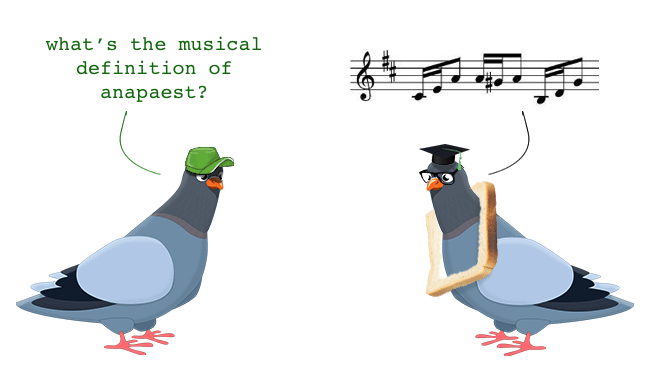
\includegraphics{anapest4.png}
\end{center}
\caption{Musical example of an anapaestic rhythm.}
\end{figure}
    Immediately, it is important to note that the two keys in which Bach has
set these subjects to are both meantone keys, a and c, as opposed to the
Pythagorean keys connected to the slow semitones. As we observed in the
previous chapter, the temperamental construction of the meantone minor
group keys (which mirror the tradition of meantone tuning), is
characterized by thirds that are closer to pure and wider semitones that
result in a mellower minor mode, one that is more associated with the
affect of softness, tenderness, and seriousness, rather than sadness,
grief, and the extremity of emotion that characterized Pythagorean minor
mode. Fittingly, the setting of the semitone as a decorative, mordant
motif in a dancelike setting gives way to a minor mode that is energetic
and elegant in character.

At this point, we will look at the type of semitone that is used for the
opening interval of the initial subject statement:

\begin{Verbatim}[commandchars=\\\{\}]
    file  cents  sc degree L directed name subject  subject offset  measure
264  c\_1    108         11.0           m-2    True             0.0        1
\end{Verbatim}
\begin{Verbatim}[commandchars=\\\{\}]
    file  cents  sc degree L directed name subject  subject offset  measure
634  a\_1     96         11.0           m-2    True             0.0        1
\end{Verbatim}
    For the c minor fugue, the widest available semitone at 108 cents is
employed; for a minor though, the semitone is narrower, at 96 cents
(second most narrow semitone available). However, there is more
complexity in the a minor fugue that needs to be accounted for: namely,
the transposition within its subject motif repetition up a third (the
reiterations of the motif within the subject in c minor retains the
pitch), and its fugue containing the subject in inversion with a full,
complete counterexposition and development of this inverted subject.

The two tables below take these items into effect; for c minor the other
two reiterations of the semitone motif within the subject (because they
are exact repetitions though, they do not present any variation), and
more importantly, for a minor, the second, transposed reiteration of the
semitone motif within the subject (transposed up a third) in the second
row entry, and the opening interval of the first statement of the
inverted subject (inverted semitone motif starting on the fifth scale
degree) in the third row entry. The second, transposed reiteration of
the subject in inverso is not included here because it happens to
outline a major second instead of a minor second. For the a minor table,
note the subject offset and directed name column in the third row entry
to verify the inverted subject statement (first statement happens on
measure 14).

\begin{Verbatim}[commandchars=\\\{\}]
    file  cents  sc degree L directed name subject  subject offset  measure
264  c\_1    108         11.0           m-2    True             0.0        1
269  c\_1    108         11.0           m-2    True             2.0        1
274  c\_1    108         11.0           m-2    True             4.0        2
\end{Verbatim}



\begin{Example}[H]
    \begin{center}
    \adjustimage{max size={0.9\linewidth}{0.9\paperheight}}{analysis_3_files/analysis_3_108_0.png}
    \caption[A minor fugue subject in inverso (mm. 14-16). ]{ A minor fugue subject in inverso (mm. 14-16). Subject starts on the pickup to the fourth beat in the first measure of the excerpt.}
    \end{center}
\end{Example}
    
\begin{Verbatim}[commandchars=\\\{\}]
    file  cents  sc degree L directed name subject  subject offset  measure
634  a\_1     96         11.0           m-2    True             0.0        1
639  a\_1    108          2.0           m-2    True             2.0        1
104  a\_1    108          7.0            m2    True             0.0       14
\end{Verbatim}
    Looking at the a minor table with the additional iterations of the
subject motif taken into account, we observe that the widest semitone at
108 cents is utilized in both cases of the reiteration of the subject
motif, and the opening of the subject inverso. While it is remains true
that the very first statement of the subject motif in recto occupies a
place of heightened importance and impact, these other presentations of
the subject motif---especially the subject inverso---are of
collective tantamount importance when it comes to the unfolding of the
character of the piece as a whole, as they altogether comprise the full
development and realization of the subject theme.

As with the previous subsection, we will now turn to examine the
distribution of all instances of the semitone subject motif for both
fugues as a function of cents. As a note: I am assigning each iteration
of the mordent motif as one count, not two. This mention is just to
clear up any potential confusion, as technically the mordent motif
contains two instances of the semitone, if one counts the descending and
ascending motion separately. Either way, this would only increase the
count number, but would not modify what we are interested in, which is
the ratios of each interval and its relationship to the others, and the
overall shape of the distribution. Finally, I have offered two charts
for the a minor fugue, one chart which includes only the opening
iteration of the subject mordent motif, and the second chart containing
all instances of the subject mordent motif.



    \begin{center}
    \adjustimage{max size={0.6\linewidth}{0.9\paperheight}}{analysis_3_files/analysis_3_112_0.png}
    \end{center}
    

    \begin{center}
    \adjustimage{max size={0.9\linewidth}{0.9\paperheight}}{analysis_3_files/analysis_3_113_0.png}
    \end{center}
    
    Observations:

\begin{itemize}
\tightlist
\item
  The results for the c minor fugue are quite straightforward, with a
  strong predilection towards the widest semitone of 108 cents, and a
  small portion of the remaining semitones at the second widest width
  available of 102 cents.
\item
  When considering only the opening motif for the a minor fugue (subject
  recto and inverso), we can see two roughly bimodal peaks at 96 cents
  and 108 cents, respectively, with a mild predilection towards 96
  cents, its count outnumbering the count of semitones at 108 cents by
  roughly 20\%. There are, as expected in the key of a minor, no
  instances of the Pythagorean limma. However, when considering all
  statements of the subject motif as a whole (essentially, counting the
  second iteration of the mordant motif), the distribution shows a clear
  predilection towards the semitone at 108 cents.
\end{itemize}

\subsection{Subsection Comparison and
Conclusions}\label{subsection-comparison-and-conclusions}

On a whole, when considering the fast, mordant semitone subject motif as
a whole, there exists a predilection towards the widest semitone
available at 108 cents, which is directly opposite of the trend observed
by the slow moving semitone motif, which showed a strong disposition
towards the narrow Pythagorean limma.


    \begin{center}
    \adjustimage{max size={0.9\linewidth}{0.9\paperheight}}{analysis_3_files/analysis_3_115_0.png}
    \end{center}
    
    Just through this section's comparison of the usage and approach to the
semitone as thematic material, we can see a clear division between theme
type and choice of key and tempered interval. Essentially when
controlling only for duration, we witness a division of two groups of
very different semitone themes with contrasting characters, each group
with a systematic key group and temperament scheme, the results of which
are comprehensively summarized in the table below:
\begin{table}[H]
\begin{singlespace}
\small
\centering
\begin{tabularx}{5.5in}{|>{\RaggedRight}X|>{\RaggedRight}X|>{\RaggedRight}X|}
\hline
                                  & \textbf{ ≥ Quarter-Note \newline Subject Semitone} & \textbf{16th-Note \newline Subject Semitone} \\
\hline
\vspace{-1em}
\begin{itemize}[leftmargin=0cm]
    \item[] \textbf{Motif Type (Pitch):                          }
    \item[] \textbf{Motif Type (Rhythm): \newline ~              }
    \item[] \textbf{Motivic \newline \mbox{Character/Traits}:    }
    \item[] \textbf{Key Group:                                   }
    \item[] \textbf{Keys:                                        }
    \item[] \textbf{Most common semitone \newline type in cents: }
\end{itemize}

                                  &

\vspace{-1em}
\begin{itemize}[leftmargin=*]
\item Cross
\item Straight \newline (no rhythmic scheme)
\item Dirge, lamenting, \newline chromatic
\item Pythagorean
\item F minor, C\# minor
\item 90 (Pythagorean limma)
\end{itemize}
                                  &

\vspace{-1em}
\begin{itemize}[leftmargin=*]
\item Mordent
\item Anapaest \newline ~
\item Driving, energetic, \newline rhythmic
\item Meantone
\item C minor, A minor
\item 108
\end{itemize}

\\

\hline
\end{tabularx}
\small
\end{singlespace}
\caption{Opening Semitone Comparison Chart}
\end{table}
    All in all, this is a demonstration of the vast variation of characters
within minor modes, and how temperament plays an important role in their
creation. In the case of these fugues that we have analyzed in this
section, the compositions' artistic integrity and musical affect is
mirrored in the temperament layout of the particular key that they are
set in and their subject semitone motifs, with the type of semitone
employed an important factor in supporting and accentuating the overall
characters of the pieces. For the slow moving, highly emotive semitone
themes, the narrow Pythagorean limma adds further intensity to the
already heightened chromatic setting of this subject type, as well as
further aiding the dissonance and depressive tendency of the interval,
whereas placing the wide semitone at 108 cents in its stead would
significantly decrease these effects. On the other hand, for the fast,
mordent semitone motif, the usage of the wide semitone helps create more
of a sense of space and stateliness of the figure, as well as provides
the performer with a greater control over the energy of the piece; the
narrow Pythagorean limma in this instance would generate too much
tension and nervous energy for this quick, ornamental like context.

Thus, while the two groups of fugues in this section use the semitone as
central subject material, the musical character and emotion conveyed is
clearly different, which is systematically reflected through the clean
division between meantone and Pythagorean, as well as the type of
semitone motif and tempering employed. Through the example of this
section, we can clearly see how the setting of the key is not merely
incidental, but intentional and purposeful, and a crucial element that
contributes actively to a pieces' overall character.

    \section{Minor Ninth (Compound Semitone) as Thematic
Material}\label{minor-ninth-compound-semitone-as-thematic-material}

This companion section of analysis to the thematic semitones will focus
upon the minor ninth---a compound semitone---as subject and
thematic material. This interval, which is part of the semitone class of
intervals, retains the attributes of heightened dissonance and
direction, but its added sonic distance makes it an unusually colorful
interval that is associated with madness (Wessel, 1955), as well as
despair (Kirnberger, 1782). Coupled with the fact that this compound
interval poses a sizable leap on the horizontal domain, this interval is
used sparingly throughout the WTC; in fact, excluding the b-flat minor
fugue, in which this interval plays a major thematic role as part of the
fugue's subject, the minor ninth only appears 7 times in the entire body
of the minor fugues of the WTC I.

All the minor fugues in which this interval makes an appearance (in
subject and non-subject material alike, and regardless of its importance
on the thematic domain) are f minor, b-flat minor, g-sharp minor,
f-sharp minor, and a minor (verified below).

    \begin{Verbatim}[commandchars=\\\{\}]
{\color{incolor}In [{\color{incolor}42}]:} \PY{n}{d}\PY{o}{=}\PY{n}{m\PYZus{}hz\PYZus{}concat\PYZus{}wk}
         \PY{n}{df}\PY{o}{=}\PY{n}{d}\PY{p}{[}\PY{p}{(}\PY{n}{d}\PY{p}{[}\PY{l+s+s1}{\PYZsq{}}\PY{l+s+s1}{name}\PY{l+s+s1}{\PYZsq{}}\PY{p}{]}\PY{o}{==}\PY{l+s+s1}{\PYZsq{}}\PY{l+s+s1}{m9}\PY{l+s+s1}{\PYZsq{}}\PY{p}{)}\PY{p}{]}
         \PY{n}{df}\PY{o}{.}\PY{n}{index}\PY{o}{.}\PY{n}{unique}\PY{p}{(}\PY{n}{level}\PY{o}{=}\PY{l+m+mi}{0}\PY{p}{)}
\end{Verbatim}
\begin{Verbatim}[commandchars=\\\{\}]
{\color{outcolor}Out[{\color{outcolor}42}]:} Index(['f\_1', 'fsh\_1', 'gsh\_1', 'a\_1', 'bfl\_1'], dtype='object')
\end{Verbatim}
    An initial, simple observation of this list is that 4 out of the 5 keys
that contain this interval belong to the Pythagorean class of keys.
While this interval does make an appearance in the above five keys
though, in the most case they do not constitute general thematic
material, and in the case of the the fast and moving sixteenth notes in
the a minor fugue, they appear as mere linear connectors dictated by the
functional need for the moving line to stay within a reasonable vocal
range. The only two fugues that use this interval as thematic material
in the entire WTC I are f minor and b-flat minor, with b-flat minor
being the only fugue that uses this special interval as subject material
in the form of an ascending leap. In contrast, the f minor fugue
utilizes the descending version of the leap as countersubject material,
however, this only makes an appearance 3 times throughout the piece,
while the subject ascending leap in the b-flat minor fugue appears 9
times.

For the analysis of this section, I will be drawing a distinction
between ascending and descending incidents of this interval and
analyzing the two groups separately, as the wide spacing of the interval
gives the two very different functional and affective roles. Also in
line with the focus of this chapter, I will mainly be looking at
incidents of this interval in a thematic context. The following is the
breakdown of this section:

\begin{enumerate}
\def\labelenumi{\arabic{enumi}.}
\tightlist
\item
  Focus upon the ascending minor ninth leap, specifically within the
  context of the b-flat minor fugue subject.
\item
  Focus upon the descending minor ninth leap, specifically within the
  context of the f minor fugue countersubject.
\end{enumerate}

    \subsection{Ascending Minor Ninth Leap (B-flat Minor
Fugue)}\label{ascending-minor-ninth-leap-b-flat-minor-fugue}

The b-flat minor fugue is uniquely the only fugue that contains the
interval of the minor ninth leap in its subject (shown below, along with
the first statement of the subject), and it is no coincidence that this
very special and unusual interval be assigned as thematic material to
this very idiosyncratic and extreme Pythagorean exemplar key.

    \begin{Verbatim}[commandchars=\\\{\}]
{\color{incolor}In [{\color{incolor}45}]:} \PY{n}{d}\PY{o}{=}\PY{n}{m\PYZus{}hz\PYZus{}concat\PYZus{}wk}
         \PY{n}{df}\PY{o}{=}\PY{n}{d}\PY{p}{[}\PY{p}{(}\PY{n}{d}\PY{p}{[}\PY{l+s+s1}{\PYZsq{}}\PY{l+s+s1}{name}\PY{l+s+s1}{\PYZsq{}}\PY{p}{]}\PY{o}{==}\PY{l+s+s1}{\PYZsq{}}\PY{l+s+s1}{m9}\PY{l+s+s1}{\PYZsq{}}\PY{p}{)}\PY{o}{\PYZam{}}\PY{p}{(}\PY{n}{d}\PY{p}{[}\PY{l+s+s1}{\PYZsq{}}\PY{l+s+s1}{subject}\PY{l+s+s1}{\PYZsq{}}\PY{p}{]}\PY{o}{==}\PY{l+s+s1}{\PYZsq{}}\PY{l+s+s1}{True}\PY{l+s+s1}{\PYZsq{}}\PY{p}{)}\PY{p}{]}
         \PY{n}{df}\PY{o}{.}\PY{n}{index}\PY{o}{.}\PY{n}{unique}\PY{p}{(}\PY{n}{level}\PY{o}{=}\PY{l+m+mi}{0}\PY{p}{)}
\end{Verbatim}
\begin{Verbatim}[commandchars=\\\{\}]
{\color{outcolor}Out[{\color{outcolor}45}]:} Index(['bfl\_1'], dtype='object')
\end{Verbatim}


\begin{Example}[H]
    \begin{center}
    \adjustimage{max size={0.9\linewidth}{0.9\paperheight}}{analysis_3_files/analysis_3_125_0.png}
    \caption[Minor ninth in the B-flat minor fugue subject (mm. 1-3). ]{ B-flat minor fugue subject (mm. 1-3). Minor ninth leap between the notes of F and G-flat, outlined between the last note of the first measure and first note of the second measure.}
    \end{center}
\end{Example}
    
    In the previous section involving fifths and fourths, we observed
through careful analysis how centric the fifth was to the thematic
construction and structure of this fugue. Tantamount though to the
importance of the perfect interval to the harmonic and structural
integrity of this piece is the minor ninth, which in some ways is the
bedrock of the coloristic identity and encapsulates the heightened
expressivity of not only this fugue, but the key of b-flat minor on a
larger scale. In this sense, the leap of the minor ninth is more closely
tied to the unique artistic identity of this fugue in that it quite
literally sets it apart from the other fugues; while the fifth is the
opening interval to this fugue, and legitimately constitutes the
foundation to the harmonic and formal structure of the piece, the first
and foremost interval still that comes to mind when recalling this fugue
is this iconic gesture of the beautiful reaching minor ninth, in all its
quiet desperation, and it is this interval that is cemented in our minds
as being inextricably tied to this fugue. David Ledbetter notes of this
relationship between this interval and key eloquently: "What appealed to
Bach in this genre was the expressive tension possible between the
objective control inherent in the \emph{stile antico} and the tortured
personal anguish of the second-practice dissonance, enhanced by the
weird key (b-flat minor)."

At the conclusion of the previous chapter, we were able to see how the
temperament profile of b-flat minor (maximum purity of perfect
intervals, and maximization of usage of extreme narrow Pythagorean
thirds and Pythagorean limma due to placement at important scalar
positions) not only makes it an exemplar Pythagorean key, but created a
minor key of extremities, and earlier in this chapter, we observed how
Bach selected this specific key, along with its sister exemplar
Pythagorean key of d-sharp minor to set the two subjects with opening
fifths in order to utilize to the greatest extent the extreme purity of
these perfect intervals. Following this logic, and our growing thesis of
Bach's sensitivity to temperament within key and the selection of
thematic intervals, we should expect to see a similar type of
correlation between the thematic minor ninth leap and a type of interval
idiosyncratic to this key and key group---the Pythagorean limma.

The following data below provides in order: 1. Table of the first
appearance of this interval found in the first subject statement of the
fugue and examine it for the specific tempering of this minor ninth 2.
Distribution of minor ninth leap in all subjects as a function of
temperament 3. Distribution of minor tenth leap in all subject answers
as a function of temperament 4. Distribution of minor ninth leap and all
descending semitone resolutions in subjects as a function of temperament
5. Distribution of subject and answer leap (both minor ninth and minor
tenth) and descending semitone resolutions as a function of temperament

\begin{Verbatim}[commandchars=\\\{\}]
    file  cents  sc degree L directed name subject  subject offset  measure
1  bfl\_1     90          7.0            m9    True             2.0        1
\end{Verbatim}


    \begin{center}
    \adjustimage{max size={0.6\linewidth}{0.9\paperheight}}{analysis_3_files/analysis_3_129_0.png}
    \end{center}
    


    \begin{center}
    \adjustimage{max size={0.6\linewidth}{0.9\paperheight}}{analysis_3_files/analysis_3_131_0.png}
    \end{center}
    


    \begin{center}
    \adjustimage{max size={0.6\linewidth}{0.9\paperheight}}{analysis_3_files/analysis_3_133_0.png}
    \end{center}
    


    \begin{center}
    \adjustimage{max size={0.6\linewidth}{0.9\paperheight}}{analysis_3_files/analysis_3_135_0.png}
    \end{center}
    
    The observations from these graphs and tables are as follows:

\begin{itemize}
\tightlist
\item
  The first instance of the minor ninth leap in the fugue is the
  narrowest Pythagorean limma (semitone at 90
  cents\footnote{In terms of cents, I am representing the compound minor ninth intervals here as their simple semitone counterparts. In reality, the total cents of the minor ninth is 1290 (semitone + octave), but using the simplified semitone cent values help for consistency of comparison and visualization.}).
\item
  70\% of all subject minor ninth leaps are the narrow Pythagorean
  limma; the rest of them utilize the second narrowest available
  semitone at 96 cents.
\item
  Because the subject evokes a perfect interval at its opening, the
  answer is tonal, causing statements of the answer of the subject to
  outline a minor tenth (compound minor third) instead of our original
  minor ninth. While the interval is different, the principle of
  preserving narrowness in the interval is retained, with all but one of
  the 7 tenths being the narrowest Pythagorean minor third, another
  interval that is idiosyncratic to the Pythagorean class keys, and to
  the exemplar keys specifically. The one other minor tenth that does
  not use the Pythagorean minor third uses the second most narrow
  variety at 300 cents. In more detail, the one occasion that a
  Pythagorean minor third is not outlined is when the subject is
  presented at the opening of the second exposition (b. 25). The subject
  is presented in its real form, first outlining D-flat major with the
  opening fourth (key area III, because of the elided cadence with the
  ending of the first exposition), but the descending sequences of notes
  after the leap immediately return back to the key area of B-flat
  minor, thus beginning on c-natural, resulting in a subject statement
  that outlines the minor tenth. However, this leap can be seen as more
  of a break rather than a continuous motion, as it essentially acts as
  a divider between the two halves of this subject statement, which is
  in a different key than the second half.
\item
  Important to the affect of this minor ninth leap motif is its semitone
  resolution down, underscoring the depressive nature of this theme.
  When considering the semitone resolution along with the leap, we can
  see that most of these semitone class intervals are Pythagorean limmas
  (74\%), and when we consider the subject gesture (upwards leap,
  semitone resolution) as a whole in the last graph, we observe that
  76\%.5 percent of these intervals belong to the narrowest of their
  class, either Pythagorean limmas, or Pythagorean minor thirds, both at
  -22 cents from just.
\end{itemize}

All in all, the overall conclusion of this subsection is clear: the
predilection for the Pythagorean limma in the context of this subject
minor ninth and semitone motif is unequivocal, as is the predilection
for the narrow Pythagorean third for the modified tenth leap in the
subject's answer. In this case, as in the case with the fifth, the usage
of the narrow limma is not just rote, but rather serves an important
role in a subject theme that relies upon the narrowness and dissonance
of the semitone class interval to enhance the difficulty of the reach
upwards, and resignation and pathos in the downwards semitone resolution
that follows, a well as to highlight the unusual chromaticism of this
special interval. Again, in the same way that we observed c-sharp minor
to be the optimal key for its unique subject construction and thematic
intervals, b-flat minor is likewise its fugue's own optimal key as well
in consideration of the importance of its two crucial subject themes and
their intended musical attributes: the maximization of the purity of the
fifth for resonance and sonority, and the narrowness and dissonance of
the minor ninth as a symbol of pathos and expressive chromaticism. The
transpositions of both subject thematic intervals/gestures (fifth,
followed by minor ninth/semitone) into all twelve minor keys are
presented in the charts below for verification:


    \begin{center}
    \adjustimage{max size={0.9\linewidth}{0.9\paperheight}}{analysis_3_files/analysis_3_137_0.png}
    \end{center}
    

    \begin{center}
    \adjustimage{max size={0.9\linewidth}{0.9\paperheight}}{analysis_3_files/analysis_3_138_0.png}
    \end{center}
    
    From these charts, we can observe that, on average, b-flat minor is the
key that greatest preserves both the purity for the thematic perfect
intervals, as well as the the narrowness (through the Pythagorean limma
and Pythagorean minor third) of the minor ninth/tenth and semitone
motif. Further observe here that the meantone class keys are all quite
abysmal, as they essentially invert the desired results - the average
exemplar meantone key of d minor being the most unfavorable. The only
other sensible contenders are its upper and lower fifth neighbor keys of
d-sharp and f minor, each actually performing slightly better for
alternating interval categories than our original key of b-flat minor
(d-sharp is the only key which perfect interval purity is slightly
better than b-flat minor, and f minor is the only key that has a higher
percentage of Pythagorean limma/third usage. However, where each of
these two keys excel in one interval domain, they lack in the other, and
quite dramatically so: while d-sharp minor may have slightly better
purity values in perfect intervals than b-flat minor, the retention of
the Pythagorean limma/third is only at 29\%, a large enough dip to make
this key unfavorable for the themes of this particular fugue. F minor
does do better on the minor ninth/semitone domain than b-flat minor, but
worse in the domain of fifths, and more importantly, the purity level on
the vertical domain of these perfect intervals between the keys of
b-flat and f minor just decreases so drastically because of the boundary
between f and c minor (a staggering difference of around 20\% in terms
of expected purity percentages for these two keys) that further make f
minor an unsuitable candidate for the richness of the five-voice fugal
texture.

As a result, b-flat minor emerges as the overall optimal choice for
maximization of the specific musical traits necessary for the themes of
its fugue at hand, and again, from focusing on subject and thematic
analysis, we observe yet another case of a composition that was written
for its exact key, and realizing it in any other would pose a compromise
to the artistic integrity and unique expressive forces of its themes,
sonic landscape, and structural architecture.

One last word on the usage of the minor ninth in the b-flat minor fugue,
while the ascending minor ninth is used as thematic subject material,
and appears consistently throughout the piece, the descending minor
ninth makes one singular appearance in the fugue (m.72, or third to last
measure in the excerpt below, bass voice):



\begin{Example}[H]
    \begin{center}
    \adjustimage{max size={0.9\linewidth}{0.9\paperheight}}{analysis_3_files/analysis_3_141_0.png}
    \caption[Descending minor ninth in b-flat minor fugue (mm. 70-74). ]{ Descending minor ninth in b-flat minor fugue (mm. 70-74). Descending minor ninth starting at pickup to m. 72, bass voice.}
    \end{center}
\end{Example}
    
    While this single appearance cannot constitute motivic material, its
presence within the piece is structurally important, and far from
casual, or merely dictated by contrapuntal or linear necessity because
of its careful placement within the composition. Bach's specific usage
of this one descending minor ninth attests to his intense attention to
detail as well as large scale structure, and his ability as a sonic
architect, as everything about its placement is symmetrical on multiple
levels, for reasons stated below:

\begin{itemize}
\tightlist
\item
  The descending minor ninth happens at the very end of the piece (3
  measures from the end), specifically after every statement of the
  ascending minor ninth has transpired. To conclude this palindromic
  effect, the following final two notes of the piece in the bass voice
  are an ascending fourth F to B-flat, a mirror of the opening
  descending fourth B-flat to F subject statement.
\item
  The descending minor ninth occurs in the bass (lower most) voice,
  while the first statement of the subject ascending minor ninth is
  stated in the soprano (upper most) voice.
\item
  The starting pitch of the interval is F, the same note as the starting
  note of the original subject ascending ninth. From that pitch, the
  subject ascending ninth reaches up to an F\#; the descending ninth
  falls down to an E.
\item
  The descending minor ninth is approached by a rising semitone, again
  mirroring the subject ninth, which is resolved by a descending
  semitone.
\end{itemize}

All these elements above concerning the pitch, presentation, placement,
and tessitura of this descending minor ninth share a systematic
symmetrical relationship to the subject ascending ninth, but the final
punchline here lies in the fact that even the tempering of this interval
is a foil to the ascending interval, as it uses the widest semitone
available at 108 cents:

\begin{Verbatim}[commandchars=\\\{\}]
      file  cents  sc degree L directed name subject  subject offset  measure
805  bfl\_1    108          6.0           m-9   False             0.0       72
\end{Verbatim}


    \begin{center}
    \adjustimage{max size={0.6\linewidth}{0.9\paperheight}}{analysis_3_files/analysis_3_145_0.png}
    \end{center}
    
    Aside from this interval's contribution to the fugue's structural
balance and symmetry, the tempering of this descending is artistically
salient, in that it further sets this descending version of the interval
apart from all of the previous thematic ascending ninths. The contrast,
boosted through temperament, is especially striking; in light of the
subject's upward gesture that seems to barely graze at the note right
about the octave before being immediately pulled downward in a sigh
motif, an effect of pathos that is magnified by the depressive
Pythagorean limma and repetition, the wide semitone used for this final
downward leap would present this interval to be positively chasmic as
well as decisive in its succinctness, adding to the color and drama of
this particular fugue.

    \subsection{Descending Minor Ninth Leap (F Minor and A Minor
Fugue)}\label{descending-minor-ninth-leap-f-minor-and-a-minor-fugue}

To close out this section, we will look at the descending minor ninth as
thematic material; contiguously, this interval as thematic material is
even rarer than the ascending minor ninth, and does not even make an
appearance in any of the fugal subjects in any of the minor fugues in
the WTC I. In fact, this interval only occurs 5 times throughout all the
minor fugues, one of which is the purposeful occurrence in the b-flat
minor fugue (analyzed above), and another in the g-sharp minor fugue,
which happens to be more incidental, and dictated by linear direction
and function, rather than carefully set up as an interval to be
highlighted. The remaining three instances occur in the countersubject
material of the f minor fugue, and the only place in which this rare
interval is used as thematic material. The first and second instances of
this countersubject is shown below (in the tenor against the subject in
the alto, and then continued in the alto, with the subject entry in the
bass):



\begin{Example}[H]
    \begin{center}
    \adjustimage{max size={0.9\linewidth}{0.9\paperheight}}{analysis_3_files/analysis_3_149_0.png}
    \caption[Countersubject descending ninths in f minor fugue (mm. 4-7). ]{ Countersubject descending ninths in f minor fugue (mm. 4-7), first and second instances of statement. First statement outlined in tenor voice against the subject in the alto (first measure of excerpt), second instance outlined in the alto, with the subject entry in the bass (fourth measure of excerpt).}
    \end{center}
\end{Example}
    
    Recalling the scale degree breakdown and analysis of the key of f minor
in the previous chapter, we observed f minor to be a boundary key with
polarizing effects when it comes to the key's chromatic layout as
dictated by the well-tempered system, as it simultaneously contains both
the Pythagorean limma and the widest semitone at 108 cents at prominent
scale degrees, creating a variegated and uneven scalar terrain. This
contrasting and uneven nature of the key's chromatic scale is reflected
in the jagged treatment of the fugue's chromaticism and juxtaposition of
intervals in its subject, which we have already analyzed in part in a
previous subsection dealing with semitones, with a slow, sinuous
semitone opening motif, punctured with the awkward leap of an ascending
perfect fourth of peculiar chromatic configuration, followed immediately
with a perfect fifth leap in the opposite direction, before continuing
with the chromatic line downwards towards a resolution on the tonic.

What is notable here is that the countersubject also reflects this same
type of roughness in the chromatic line through the sudden and jolting
descending minor ninth leap, placed awkwardly within an otherwise smooth
rising group of stepwise figures. So, while this minor ninth occurs as
countersubject material, it is nonetheless an important continuation to
the subject theme, both gesturally and coloristically through
juxtaposition of chromatic leaps against chromatic smoothness,
representing the difficult and polarizing nature of the chromaticism in
this particular key. Let us consider the tempering of the three
instances of this interval:

\begin{Verbatim}[commandchars=\\\{\}]
     file  cents  sc degree L directed name  measure
359   f\_1    108         11.0           m-9        7
728   f\_1    108          6.0           m-9        4
1154  f\_1    108         11.0           m-9       13
\end{Verbatim}


    \begin{center}
    \adjustimage{max size={0.6\linewidth}{0.9\paperheight}}{analysis_3_files/analysis_3_153_0.png}
    \end{center}
    
    All of the three iterations of this countersubject descending minor
ninth leap are at the widest semitone value of 108 cents, consistent
with the same width as the descending minor ninth statement in the
b-flat minor fugue. In the specific context of the chromaticism in this
particular fugue, the enhancement of this wide distance through the
usage of the semitone at 108 cents musically accentuates this awkward
interruption of the line, creating even more of a disruptive effect to
the smooth, upward creeping line that forms the rest of the
countersubject material.

Even though the statements of the minor ninth interval---ascending
and descending---are rare occurrences across the collection of
fugues, an overwhelming majority of the interval's usage is in important
thematic (either subject or countersubject) material. In fact, out of
the 13 statements of the ascending ninth, 10 are thematic (subject
ninths in b-flat minor), and out of the 5 descending ninths, 4 are
thematic, with 3 belonging to the f minor countersubject, and the
remaining one belonging to the single symmetric statement at the
conclusion of the b-flat minor fugue. With this in consideration, it is
clear that Bach is not merely avoiding this interval, or relegating it
to haphazard usage or employment out of contrapuntal necessity. Rather,
the presence of this interval in these fugues is due to careful and
thoughtful planning, its thematic usage dictated by aesthetic decisions
based on the interval's sonic properties and expressive implications,
and how these unusual coloristic properties are able to aid the musical
integrity of the larger composition. This is further bolstered through
the systematic consistency of tempering on the directional domain of
this interval, as we were able to observe a clear and systematic
consistency in the division between the assignment of the narrow
Pythagorean limma to the ascending minor ninth, and the wide 108 cent
semitone for the descending minor ninth. The summary these minor ninth
are presented in the graphs below, the first set summarizing the
thematic ninth intervals that we've analyzed in this section, and the
second set containing all instances of minor ninths regardless of
thematic usage.


    \begin{center}
    \adjustimage{max size={0.9\linewidth}{0.9\paperheight}}{analysis_3_files/analysis_3_155_0.png}
    \end{center}
    

    \begin{center}
    \adjustimage{max size={0.9\linewidth}{0.9\paperheight}}{analysis_3_files/analysis_3_156_0.png}
    \end{center}
    
    While we have shown through this section's analysis the larger, musical
significance of the tempering of these intervals in context of their
compositions, beyond the specific thematic import attached to
composition, there could be deduced something of a general natural
effect occurring here in regards to the difference between the tempering
of these intervals as a function of direction. In this sense, if one
were to translate the sonic space of these intervals into the physical
space, with ascension akin to upward direction, and descent downward, it
would follow that the difficultly of the minor ninth upward reach would
be further supported by a narrower interval, highlighting the natural
strain against gravity of this motion. On the other hand, a minor ninth
plunge would naturally call for a wider interval to abet the natural
trajectory of this fall. The fact that this connection between interval
direction and specific tempering is preserved by Bach in his thematic
usage of the minor ninth provides us with a beautiful example of the
power that these tempered intervals exert on the domain of musical
expression, and how this can be positively reflected in composition.

Finally, something can to be said about the two keys that contain these
thematic minor ninths: they are both Pythagorean keys, and given that
the minor ninth is an unusual interval in its expressive color and
force, it would makes sense that this interval would be associated with
and utilized by the more unusual and extreme chromatic configuration and
availability of the narrow Pythagorean limma in these keys.
Interestingly though, the descending minor ninth used in both these
fugues uses the semitone at 108 cents, which is much more commonly found
in the meantone keys. This makes Bach's employment of this specific
configuration of this interval in these Pythagorean keys all the more
deliberate and meaningful, as he wasn't just haphazardly selecting an
interval that was plentiful, but rather employing this specific version
of this interval for its coloristic properties. Furthermore, both the
fugues rely simultaneously on subject material that places significant
focus upon the Pythagorean limma version of this semitone, and this
contrast between the two types of semitones serve to dramatize and
magnify the individual effects of each. Ultimately, Bach's goal in this
interval is tone color, and the accentuation of the expressive
characters of these respective keys; for the b minor fugue, casting
extreme chromatic dissonance against a backdrop of pure fifths, and in
the f minor fugue, featuring the contrasting chromatic shades that the
awkward key has to offer.

    \section{Enharmonic Equivalency and
Temperament}\label{enharmonic-equivalency-and-temperament}


    The final section of this chapter will depart a bit from the road of the
main discourse of the past chapter and a half that has been concerned
with perfect interval and semitones, and look at another possible
dimension of the subtleties of temperament as a distinguishing force
through comparing the temperamental differences between special
enharmonic and chromatic intervals against their more standard or
diatonic counterparts, in hopes to study how temperament can be used as
a further means of chromatic color, as well as a tool of harmonic
reinforcement. The first two intervals that I will be examining in this
chapter are the more unusual intervals of the diminished seventh and the
diminished fourth, and the last interval a chromatic version of the
perfect fourth, all of which are used as prominent subject material in
various minor fugues. The interesting component of all of these
intervals lie in that, although they are each enharmonically equivalent
(and in the case of the perfect fourth, actually equivalent) to
consonant intervals (d7 to M6, and d4 to M3), it is precisely their
function within the larger tonal structures of their compositions that
causes the listener to perceive of them as dissonances, a major
testament to the power of harmonic priming, and the contextual nature of
music. The goal in this section is to ascertain whether or not
temperament is systematically and measurably used as a mechanism to
reinforce the already built-in perceptions of dissonances attached to
these intervals, and how this further plays into the musical characters
and expressivity of the subjects that utilize them.

It is important to stress here that the analysis of this section is not
stating that temperament provides more harmonic context and function to
enharmonic intervals: in some ways enharmonic equivalence in our tonal
system is somewhat meaningless because tonal context and function can
usually be readily and reliably deduced from the way intervals are set
up within the tonal framework of a piece, how pitches are spelled out on
the score, how these pitches are set up and resolved, as well as which
scale degrees they outline in relationship to the tonic. However, the
point that we are trying to make with temperament is that, under an
unequal tuning system, which creates a variety of different sizes of
intervals under the same class, different sizes/degree of tempering of
the interval can be used to strengthen our perception of harmonic
function, ranging from aiding voice leading (for example, a
narrower-than-pure interval for the diminished fourth interval may aid
in the resolution of these pitches and heighten the feeling of tension
and resolution), to reinforcing a more abstract sort of affect that the
interval engenders (for example, usage of the wide, Pythagorean interval
for the diminished seventh to highlight the interval's dissonance and
dramatic distant of the interval's leap). This is something that we do
not get in a system of equal-temperament, in which each interval class
only contains one size of interval. If we can observe that Bach
consistently uses a specific size of interval in conjunction to the
interval in a specific, already determined harmonic function (for
example, the usage of the wide Pythagorean major sixth at 906 cents for
the diminished seventh), then we can begin to surmise that this was a
purposeful choice that could very well have been used to enhance some
aspect of the interval's meaning, even though we might not be able to
determine for sure what the intended effect may be. So while these
subtleties may not be technically presenting any new information that
could not have already been deduced through looking at the spelling of
the notes/voice resolution etc., in terms of harmonic function, they
definitely do exert an effect on other aspects of harmonic quality, such
as color and the motion created by tension and resolution.~

    \subsection{Diminished Sevenths vs. Major
Sixths}\label{diminished-sevenths-vs.-major-sixths}

In the more general, tonal context, the interval of the diminished
seventh is much more commonly associated with minor mode than major,
largely due to the common harmonic function of the fully diminished
seventh (vii°7) in cadential points in minor mode, its dissonance
mitigated by its powerful resolution direction. Function aside though,
the leap of the diminished seventh interval is a dramatic gesture of
dissonance that had found its place into the common idiom by the latter
seventeenth century, and subsequently utilized as thematic material in
other Bach compositions such as the harrowing Chorale Prelude Durch
Adam's Fall from the Orgelbüchlein, as well as in the subject for the
fugue in the serious Kyrie from Mozart's D-minor Requiem (in fact, the
subject from Mozart's fugue is almost identical to the fugue subject of
Bach's WTC II a minor fugue).

Talking in terms of temperament, this specific leap is notable because
its enharmonically equivalent interval, the major sixth, is the
inversion of the minor third, and the narrow Pythagorean third at 294
cents is converted into the widest type of major sixth at 906 cents,
wider than any other major sixth previously found under the meantone
system of tuning. Furthermore, the Pythagorean minor thirds (semiditone)
were originally intervals in the meantone system that corresponded with
the interval comprised of two large/wolf wholetones, it would follow
that the inverse, the major sixth, has sonic ties to some interval
vaguely reminiscent of a seventh. For this reason, looking at the
relationship between the interval of the diminished seventh and the
inverse of the Pythagorean third (wide, ``Pythagorean'' sixth, if you
will) could yield fruitful information in terms of how temperament can
enhance and reinforce the harmonic function of an enharmonic interval,
with strong, positive correlations providing affirmation towards this
belief.

Before we go on to look at the diminished seventh as subject material, I
will first compare the distribution of the diminished seventh to that of
the Major sixth in the general body of composition (i.e. not
parameterizing for subject) to see if there are any remarkable
differences between these two enharmonically equivalent intervals
outside of a specific thematic context. The distributions are presented
in the tables below, measuring normalized duration as a function of
cents, the diminished seventh marked in red, and the Major sixth marked
in blue, in this case strictly for the purpose of distinguishing the
two.


    \begin{center}
    \adjustimage{max size={0.9\linewidth}{0.9\paperheight}}{analysis_3_files/analysis_3_162_0.png}
    \end{center}
    
    From looking at the shapes of the these distributions, the clear
conclusion that we can deduce from comparing the two charts are:

\begin{enumerate}
\def\labelenumi{\arabic{enumi}.}
\tightlist
\item
  The distribution of the diminished seventh shows a strong, positive
  correlation between interval width and frequency of occurrence, with a
  large, unmistakable majority of intervals falling on the widest
  interval type at 906 cents.
\item
  This is sharply contrasted with the shape of the distribution of the
  Major sixth, which is more amorphous and shows little correlative
  effect between interval width and frequency of occurrence. Rather, the
  values are more evenly distributed amongst width values, with a
  majority of intervals occurring at the middle values.
\end{enumerate}

If we believe in a null hypothesis that harmonic context should not have
any bearing on temperament, then we should logically expect these two
sonically identical intervals to bear similar distribution shapes.
However, the fact that the opposite is true, and that the distribution
of the diminished seventh further shows such strong and systematic
correlative effects between interval width and frequency is a strong
indicator that harmonic context is a guiding factor to Bach's choice of
tempered interval choice. From these two factors in this theme-free
context, it can be inferred from the data that Bach was utilizing the
dramatically tempered, Pythagorean major sixth as a means to reinforce
and contextually strengthen the underlying harmonic function of the
diminished seventh interval. Having established this positive
relationship between interval width and harmonic context, we will now
turn to looking at this interval in a thematic/subject context:

    \subsubsection{Diminished Sevenths as Subject
Material}\label{diminished-sevenths-as-subject-material}

The diminished seventh appears as subject material in four different
fugues in the WTC I, two in the form of a contiguous interval (a minor
and b minor), and two containing the interval outlined over a skip (d
minor and g minor). The reason for the inclusion of these two instances
of these subject diminished sevenths in skip into our pool of analysis
is that in both these cases, the main interval outlined informed by the
underlying harmony is undoubtedly the diminished seventh, both pitches
which furthermore fall on upon the strong beats of the measure. There
are additionally 3 fugues in the WTC II whose subjects also include this
interval---the a minor fugue in a quite prominent fashion---but
I will continue to limit the focus to the fugues in the WTC I alone as
to preserve the consistency of the data.

Also, just as a note---the selection process for thematic intervals
within the subject for the intervals of this section (diminished
seventh, diminished fourth, chromatic fourth), as well as the minor
ninths from the previous section, has been considerably more liberal
than the fifths and semitones, the former two which I restricted to only
looking at opening intervals, and the latter which I have opened up to
all subject intervals. This is not to purposefully constrain or
influence the data, but rather motivated strictly by necessity dictated
by the tonal nature of these intervals: the fifth and the semitone are
just far too common intervals in terms of their function and ubiquity in
the tonal system, so constraining them to looking at only opening
intervals ensures for a feasible, as well as nonpartisan method to
select for thematic importance. On the other hand, the intervals of the
ninth, and other intervals of this section are rather rare, so their
presence in the subject already has a very high chance of thematic
importance, and additional further constraints besides looking at
subject/countersubject material would result in a dearth of data.

The following \texttt{music21} code corroborates the appearance of the
contiguous diminished sevenths in the a minor and b minor fugue (the
intervals by skip will not appear in this search, and rather have been
identified manually), and the subjects from the four fugues are provided
below. Proceeding, graphs of the distribution of these diminished
seventh subject intervals as a function of interval size are provided in
a table marked with red bars, and following is a table containing all
occurrences of Major sixths for those same fugues for comparison (marked
in blue).

    \begin{Verbatim}[commandchars=\\\{\}]
{\color{incolor}In [{\color{incolor}406}]:} \PY{n}{d}\PY{o}{=}\PY{n}{m\PYZus{}hz\PYZus{}concat\PYZus{}wk}
          \PY{n}{df}\PY{o}{=}\PY{n}{d}\PY{p}{[}\PY{p}{(}\PY{n}{d}\PY{p}{[}\PY{l+s+s1}{\PYZsq{}}\PY{l+s+s1}{name}\PY{l+s+s1}{\PYZsq{}}\PY{p}{]}\PY{o}{==}\PY{l+s+s1}{\PYZsq{}}\PY{l+s+s1}{d7}\PY{l+s+s1}{\PYZsq{}}\PY{p}{)}\PY{o}{\PYZam{}}\PY{p}{(}\PY{n}{d}\PY{p}{[}\PY{l+s+s1}{\PYZsq{}}\PY{l+s+s1}{subject}\PY{l+s+s1}{\PYZsq{}}\PY{p}{]}\PY{o}{==}\PY{l+s+s1}{\PYZsq{}}\PY{l+s+s1}{True}\PY{l+s+s1}{\PYZsq{}}\PY{p}{)}\PY{p}{]}
          \PY{n}{df}\PY{o}{.}\PY{n}{index}\PY{o}{.}\PY{n}{unique}\PY{p}{(}\PY{n}{level}\PY{o}{=}\PY{l+m+mi}{0}\PY{p}{)}
\end{Verbatim}
\begin{Verbatim}[commandchars=\\\{\}]
{\color{outcolor}Out[{\color{outcolor}406}]:} Index(['a\_1', 'b\_1'], dtype='object')
\end{Verbatim}


\begin{Example}[H]
    \begin{center}
    \adjustimage{max size={0.9\linewidth}{0.9\paperheight}}{analysis_3_files/analysis_3_167_0.png}
    \caption[Diminished seventh leap in a minor fugue subject (mm. 1-3). ]{ A minor fugue subject (mm. 1-3). Descending diminished seventh leap (contiguous) in second measure.}
    \end{center}
\end{Example}
    


\begin{Example}[H]
    \begin{center}
    \adjustimage{max size={0.9\linewidth}{0.9\paperheight}}{analysis_3_files/analysis_3_169_0.png}
    \caption[Diminished seventh leap in b minor fugue subject (mm. 1-3). ]{ B minor fugue subject (mm. 1-3). Two diminished seventh leaps (continuous) in second measure.}
    \end{center}
\end{Example}
    


\begin{Example}[H]
    \begin{center}
    \adjustimage{max size={0.9\linewidth}{0.9\paperheight}}{analysis_3_files/analysis_3_171_0.png}
    \caption[Diminished seventh leap (noncontiguous) in d minor fugue subject (mm. 1-3). ]{ D minor fugue subject (mm. 1-3). Ascending diminished seventh leap (noncontiguous) in second measure.}
    \end{center}
\end{Example}
    


\begin{Example}[H]
    \begin{center}
    \adjustimage{max size={0.9\linewidth}{0.9\paperheight}}{analysis_3_files/analysis_3_173_0.png}
    \caption[Diminished seventh leap (noncontiguous) in g minor fugue subject (mm. 1-2). ]{ G minor fugue subject (mm. 1-2). Descending diminished seventh leap (noncontiguous) in first measure.}
    \end{center}
\end{Example}
    



    \begin{center}
    \adjustimage{max size={0.9\linewidth}{0.9\paperheight}}{analysis_3_files/analysis_3_176_0.png}
    \end{center}
    

    \begin{center}
    \adjustimage{max size={0.9\linewidth}{0.9\paperheight}}{analysis_3_files/analysis_3_177_0.png}
    \end{center}
    
    The observations from the above data are as follows:

\begin{enumerate}
\def\labelenumi{\arabic{enumi}.}
\tightlist
\item
  For all of these fugues---especially a minor, g minor, and d
  minor, the predilection towards the widest Major sixth at 906 cents is
  unequivocally clear.
\item
  For a minor and d minor, all of the subject diminished sevenths are of
  the widest 906 variety; for g minor, 9 of the 11 intervals are at 906
  cents, with the remaining two at the second widest variety of 900
  cents. Furthermore, out of the four fugues, a minor is the fugue with
  the strongest presence of the diminished seventh in its subject, if we
  consider that the interval is presented contiguously, and b minor's
  interval is presented in a series of leaps, and is not the sole
  intervallic focus of the subject.
\item
  The fugue containing the diminished seventh with the arguably weakest
  thematic role is b minor (for reasons given in the above point), and
  the only fugue that contains intervals at the narrower 894 and 888
  cents. Nonetheless, there still exists a strong correlation between
  interval width and frequency, with the most values lying at 906 cents,
  and decreasingly smoothly as a function of width.
\item
  When comparing the distributions of diminished sevenths to the
  distribution of Major sixths for each fugue, we see a very different
  shape in the distribution, with the Major sixth interval width values
  as a whole favoring the mid-values, with very little usage of the
  widest interval at 906 cents (in the case of a minor, there are no
  instances of this interval at all). Because of these clear differences
  in distribution shapes and frequency peaks in these enharmonically
  equivalent intervals, we can observe how their distinction in harmonic
  function is clearly reinforced through the different tempering of the
  intervals, as the diminished sevenths in these keys are set apart from
  the Major sixths in these keys through being assigned to wider
  intervals.
\item
  All the fugues that utilize the diminished seventh leap are meantone
  class fugues.
\end{enumerate}

This final point about the key group of these fugues is both an
interesting and salient one, and in no way accidental when it comes to
this particular choice of key for the usage of this enharmonic interval
as prominent thematic material, and further attests to Bach's
sensitivity to the fine grained differences available to him through the
system of well-temperament. The Major sixth is the inversion of the
minor third, and as we have observed through the scale degree charts, as
well as earlier in this chapter, the narrow Pythagorean minor third (and
the inverse wide "Pythagorean" Major sixth) is an interval associated
with the Pythagorean class keys, not the meantone keys (as demonstrated
in the charts below using the example of exemplar meantone key d minor
compared with exemplar Pythagorean key b-flat minor).


    \begin{center}
    \adjustimage{max size={0.9\linewidth}{0.9\paperheight}}{analysis_3_files/analysis_3_179_0.png}
    \end{center}
    

    \begin{center}
    \adjustimage{max size={0.9\linewidth}{0.9\paperheight}}{analysis_3_files/analysis_3_180_0.png}
    \end{center}
    
    In a sort of facile way, we may initially expect these wide, 906 cents
diminished sevenths---which are enharmnonic equivalents to the
sixths---to appear in Pythagorean keys, however, because of the way
the scale is constructed in well-temperament, it turns out that it is in
fact the meantone keys that contain the wide, Pythagorean major sixth at
the appropriate scale degrees for the diminished sevenths, not the
Pythagorean keys. Given this, if Bach wanted to distinguish the
diminished seventh from the Major sixth by virtue of a wider interval,
he would have to go the route of choosing a meantone key, not a
Pythagorean key (which would actually reverse the effect) which is
exactly what we are observing here with these thematic diminished
sevenths consistently being set in a meantone keys. These fugues are
therefore apt examples of Bach systematically selecting a key class for
which the tempering would set apart the specific thematic interval from
its enharmonically equivalent counterparts to further reinforce harmonic
function and expressivity.

Lastly, I would like to expound a bit on the falling symbolism evoked by
the descending version of this interval, and more importantly, the role
that temperament may have played in establishing the larger trend of
musical symbols, and the affects and character that we have come to
associated them with. Returning to the falling symbolism in the
descending diminished seventh, the musical factors that are presumably
responsible for this imagery are the interval's joint property of
distance and dissonance, which are not unlike that of the descending
minor ninth, which shares in these similar sonic traits, and like the
diminished seventh, is represented using the widest interval size
available for its interval group. However, while the minor ninth in
context of the key and tempo settings of their fugues seem to be more
focused on conveying the affective elements of pathos and despair, the
faster tempos and meantone keys assigned to the diminished seventh
interval seem to give it more of a seriousness and severity in quality,
consistent to the overall character of the meantone minor keys that they
are found
in\footnote{Jean Rousseau describes the character of both the key of a and d minor to be "serious" (Rousseau, 1691); Marc-Antoine Charpentier uses the same term to describe d minor as well, and g minor (Charpentier, 1692).}.

Indeed, this connection between the diminished seventh and the schema of
falling, especially focused on more of a serious context, is overtly
(and in some ways, more easily) observable in the more directly
programmatic compositions outside of the WTC provided above of Bach's
Durch Adams Fall and Mozart's Kyrie. Both pieces evoke the subject of
the severity of the consequence from man's fall, the Kyrie set in a
Requiem Mass (the movement takes on the form of a fugue, and its subject
resembles closely the fugal subject from the a minor fugue in WTC II),
and is a movement of supplication for mercy upon the sins of fallen man,
and Durch Adams Fall engaging the subject quite directly as far as
evoking it in a titular manner. Excerpts from all three compostions are
listed below in respective order. In terms of the musical settings, both
are faster movements (the movement from the tempo underscoring the
dramatic severity of the fall), similar to the tempos and note durations
found in the meantone keys of the WTC I fugues, and both prominently
utilize the theme of the diminished seventh as musical symbolism for
this falling motion (observe the series of descending diminished seventh
leaps in the bass voice in the opening of Durch Adams Fall below).

    Chorale prelude - Through Adams fall D minor BWV 637 from the "Little
Organ Book" (BWV 599-644)
\begin{Example}[H]
\centering
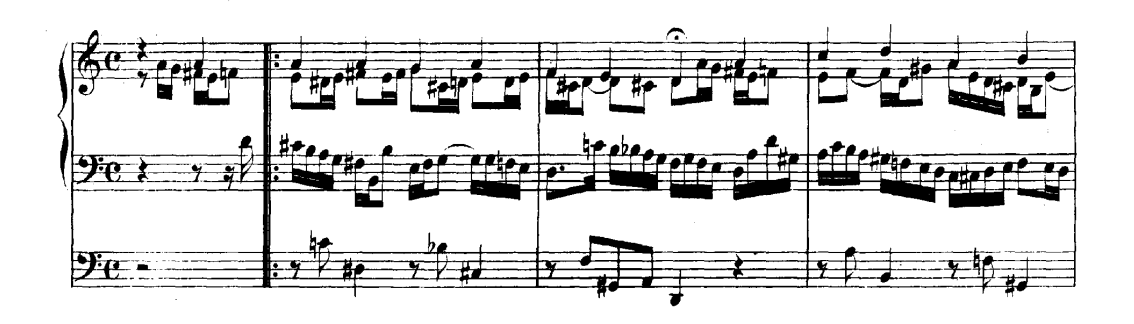
\includegraphics{durch_adams_fall_nt.png}
\caption[Opening to J.S. Bach's Durch Adams Fall (BWV 637), from the Orgelbüchlein.]{Opening to J.S. Bach's Durch Adams Fall (BWV 637), from the Orgelbüchlein (mm. 1-3). Thematic and symbolic descending diminished seventh leaps in the bass voice as musical symbolism of the fall.}
\end{Example}

\begin{Example}[H]
\centering
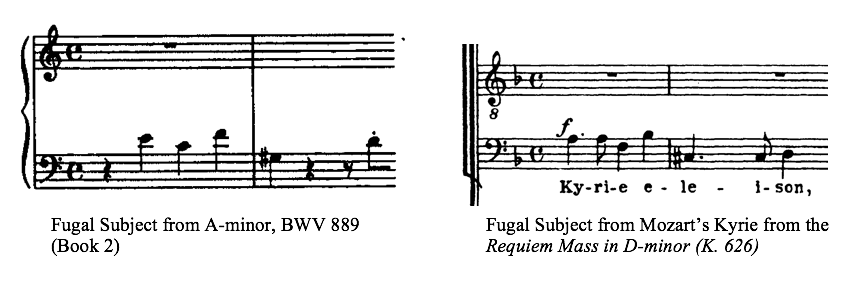
\includegraphics{kyrie_text.png}
\caption{Comparison between similar fugal subjects of Bach's WTC II a minor fugue (BWV 889) and Mozart's Kyrie from the Requiem Mass in D minor (K. 626).}
\end{Example}
    While the preludes and fugues in the WTC are not so openly programmatic,
they are equally evocative in the moods and expressions that they
convey, and we must furthermore remember that musical symbolism played
an enormous role in the conveyance of expressivity in the high Baroque
era, and certainly very much so in Bach's own expressive usage of themes
and motifs. So in this light, alongside with--and perhaps even further
than--the harmonic function that the tempering of these intervals
seeks to reinforce is the amplification of the dissonance and width of
the interval to facilitate this symbolism of the severity of the falling
motion in these diminished sevenths. Indeed for these descending
versions of the diminished seventh in the WTC I (theme invariant), the
distribution lists considerably more extremely towards the 906 cent
version of the interval (with no occurrences at the narrow version of
the interval at 888 cents), and the difference between its peak and that
of the enharmonic major sixths is markedly more pronounced than in the
directionally neutral case of the interval (as depicted in the charts
below)---altogether increasingly its musical and dramatic effect.


    \begin{center}
    \adjustimage{max size={0.9\linewidth}{0.9\paperheight}}{analysis_3_files/analysis_3_185_0.png}
    \end{center}
    

    \begin{center}
    \adjustimage{max size={0.9\linewidth}{0.9\paperheight}}{analysis_3_files/analysis_3_186_0.png}
    \end{center}
    
    Returning to this comparison between the minor ninth and diminished
seventh though: while one can question the fact as to whether the minor
ninth should be inherently associated with more morose, gloomy affects,
and the diminished seventh associated with more upbeat characters of
seriousness, what we can witness and attest to in this case is the
consistency of the symbolism in these two intervals at least throughout
the collection of the WTC I, with thematic ninths assigned to the domain
of Pythagorean keys and slower tempos, and thematic diminished sevenths
associated with the more upbeat Meantone keys and faster tempos. What
can be seen here is an interesting phenomenon perhaps akin to the
proverbial question of the chicken and egg: perchance it was something
inherent in the difference between these two intervals that motivated
their respective different key group assignments, but more likely in
this case it was the temperament that dictated key assignment, from
which then the symbolism was subsequently cemented in the common
vernacular. Certainly through our analysis of these two intervals, we
have reason to believe the latter in this case, thus making this an apt
example of temperament not only having a significant hand in the
responsibility for the character of keys, but also a major role in
dictating the certain types of affects that we associate with musical
symbols and motifs. These affects of key characteristics and musical
symbols in turn have become preserved and encoded across time through
the other musical elements that they had originally been associated
with, and thus remain in our collective musical consciousness even far
after the reign of well-temperament has given way to our modern system
of equal temperament.

    \subsection{Diminished Fourths vs. Major
Thirds}\label{diminished-fourths-vs.-major-thirds}

The next enharmonic interval that we will examine in this section is the
diminished fourth, another example of an interval that, used within its
normal harmonic context carries an extreme degree of perceived
dissonance and tension, contrasted against its enharmonic equivalent
interval of another imperfect consonance: the major third. Like the
diminished seventh in the previous section, the diminished fourth as a
functional interval is much more commonly found in minor mode, with
roughly equivalent amount of occurrences between the two across all
minor mode fugues in the WTC I (49 instances of the diminished fourth,
and 43 for the diminished seventh, compared against only 11 diminished
fourths and 10 diminished sevenths across the major mode fugues).
However, in a thematic context, the diminished fourth appears in only
one fugal subject across the WTC I minor fugues: the c-sharp minor
fugue. In this section, we will again first look at the difference
between the diminished fourth and major third in a general context,
discuss the harmonic implications of the differing shapes of the
distributions, and then proceed to unpack the usage of the diminished
fourth in the c-sharp minor fugue's subject, and how it contributes to
the subject's symbolism and overall fugue's affect and character.

Before getting into the analysis of this chapter, I will briefly discuss
the major third and its temperament scheme here to provide some
necessary background information. While we have not directly touched
much upon this interval in this dissertation due to our focus on the
minor mode, the basic tenets that we have observed of meantone vs.
Pythagorean and their respective interval purity schemes carry over and
apply to this interval as well. Like the minor third, the major third is
an imperfect consonance, and its purity is maximized by the meantone
major and minor keys, with the most extreme tempered version of this
interval (the Pythagorean major third) assigned to the remote,
Pythagorean class keys. Consistent with the temperamental layout that we
have observed in the minor keys, the relative major keys to our exemplar
minor keys of b-flat and d-sharp---C-sharp Major and F-sharp
Major---are the most extreme versions of the Pythagorean keys,
containing the Pythagorean major third at the most prominent tonal
positions of tonic and dominant. In contrast, the keys of C major and F
major (relative major to exemplar meantone minor keys a minor and d
minor) comprise our exemplar meantone major keys, containing pure thirds
at their tonally prominent locations. The key difference though between
the major third and minor third---and the main one that the reader
should keep in mind---for this section, is that the relationship
between purity and width is inverted between the two intervals, that is
to say, while the purest minor third is the widest of all variety of
thirds, the purest major third is the narrowest, mathematically dictated
by how these intervals are complements in their construction of the pure
fifth (Pythagorean 294+408=702; meantone 390+312=702).

The following is the distribution of all diminished fourths across the
minor mode fugues of WTC I (marked in blue) compared against the
distribution of the enharmonically equivalent major thirds (indicated in
red):


    \begin{center}
    \adjustimage{max size={0.9\linewidth}{0.9\paperheight}}{analysis_3_files/analysis_3_189_0.png}
    \end{center}
    
    Looking at the shapes of these two distributions, we observe the
following:

\begin{enumerate}
\def\labelenumi{\arabic{enumi}.}
\tightlist
\item
  For the chart of the diminished fourths, a decisive majority of
  intervals (60\%) fall on the narrowest---and purest
  version---of the Major third at 390 cents (only 4 cents from pure
  at 386 cents, and the purest major third offered within the system of
  well-temperament). From there, the frequency drops off sharply as a
  direct function of interval purity, with the widest, Pythagorean Major
  third at 408 cents only accounting for 5\% of the intervals.
\item
  The distributions of the diminished fourth and major third are
  remarkably different, with the diminished fourth showing strong
  positive correlative effects between interval purity (and in this
  case, narrowness) and frequency, whilst the major third distribution
  is much more uniform across the four width values, with peaks actually
  in the opposite direction at the wider, more tempered interval size of
  402 cents.
\end{enumerate}

The resulting different shapes in the distribution for these two
enharmonic intervals, as well as the strong correlative effects for the
diminished interval and its sharp preference towards the narrow/pure
version of the interval at 390 cents resembles the same type of outcome
that we witnessed with the diminished seventh in the preceding section,
again indicating that in this case as well, temperament is an important
vehicle in supporting and strengthening the differing harmonic contexts
of the two intervals. Furthermore, considering that in the well-tempered
tuning system, the 390 cent narrow and closest-to-pure Major third is
rather rare, with only 2 out of the 12 Major thirds belonging to this
category (C-E and F-A), the prominent predilection for this particular
narrow interval for the diminished fourth reflects a deliberate,
compositional decision.

Having again established a relationship between tempered interval choice
and harmonic function, we will turn our attention to the diminished
fourth as thematic material in the first subject of the c-sharp minor
fugue.

    \subsubsection{Diminished Fourth as Subject
Material}\label{diminished-fourth-as-subject-material}

The only fugue to utilize the diminished fourth in the WTC I as subject
material is the c-sharp minor fugue (first subject). We have already
analyzed this fugue and both its subjects quite intricately in two
separate previous occasions in this chapter, but here we will further
examine how the diminished fourth---in conjunction to the opening
semitone of this fugue subject---contributes further depth to the
musical character of the subject's symbol of the cross, as well as the
overall character and affect of the fugue's key. Below we have
corroborated the presence of the diminished fourth in (and only in) the
c-sharp minor fugue for book I, as well as displayed the subject.
Following immediately is a table detailing the first statement of the
interval's cent value, and a table of graphs looking at the distribution
of all subject diminished fourths (marked again in blue) compared
against the distribution of all major thirds in the fugue (marked in
red).

    \begin{Verbatim}[commandchars=\\\{\}]
{\color{incolor}In [{\color{incolor}57}]:} \PY{n}{d}\PY{o}{=}\PY{n}{m\PYZus{}hz\PYZus{}concat\PYZus{}wk}
         \PY{n}{df}\PY{o}{=}\PY{n}{d}\PY{p}{[}\PY{p}{(}\PY{n}{d}\PY{p}{[}\PY{l+s+s1}{\PYZsq{}}\PY{l+s+s1}{name}\PY{l+s+s1}{\PYZsq{}}\PY{p}{]}\PY{o}{==}\PY{l+s+s1}{\PYZsq{}}\PY{l+s+s1}{d4}\PY{l+s+s1}{\PYZsq{}}\PY{p}{)}\PY{o}{\PYZam{}}\PY{p}{(}\PY{n}{d}\PY{p}{[}\PY{l+s+s1}{\PYZsq{}}\PY{l+s+s1}{subject}\PY{l+s+s1}{\PYZsq{}}\PY{p}{]}\PY{o}{==}\PY{l+s+s1}{\PYZsq{}}\PY{l+s+s1}{True}\PY{l+s+s1}{\PYZsq{}}\PY{p}{)}\PY{p}{]}
         \PY{n}{df}\PY{o}{.}\PY{n}{index}\PY{o}{.}\PY{n}{unique}\PY{p}{(}\PY{n}{level}\PY{o}{=}\PY{l+m+mi}{0}\PY{p}{)}
\end{Verbatim}
\begin{Verbatim}[commandchars=\\\{\}]
{\color{outcolor}Out[{\color{outcolor}57}]:} Index(['csh\_1'], dtype='object')
\end{Verbatim}


\begin{Example}[H]
    \begin{center}
    \adjustimage{max size={0.9\linewidth}{0.9\paperheight}}{analysis_3_files/analysis_3_194_0.png}
    \caption[Diminished fourth in c-sharp minor fugue first subject (mm. 1-3). ]{ C-sharp minor fugue first subject (mm. 1-3). Diminished fourth in second measure.}
    \end{center}
\end{Example}
    
\begin{Verbatim}[commandchars=\\\{\}]
       file  cents  sc degree L  measure subject  subject offset
1171  csh\_1    390         11.0        2    True             4.0
\end{Verbatim}

    \begin{center}
    \adjustimage{max size={0.9\linewidth}{0.9\paperheight}}{analysis_3_files/analysis_3_196_0.png}
    \end{center}
    
    The immediate observations of the data are as follows:

\begin{itemize}
\tightlist
\item
  The predilection for the narrowest (and purest) interval at 390 cents
  for the thematic diminished seventh is unequivocal, with 76\% of the
  intervals falling on this type, and no occurrences of the Pythagorean
  interval at 408 cents. This trend is considerably more dramatic in the
  case of this individual fugue than in the general case observed
  before.
\item
  The contrast between the diminished fourth and enharmonically
  equivalent major third distribution is very pronounced; while the
  diminished fourths mostly employ the narrowest interval at 390 cents,
  the thirds are comprised of the wider intervals of 402 cents and the
  Pythagorean major third, with no occurrences at the narrower 396 and
  390 cents. This polarization of the two enharmonically equivalent
  intervals is even more dramatic than in the case of the general
  (thematically neutral) intervals, and is undoubtedly partially due to
  the key of c-sharp minor that the fugue is set in, which we determined
  to be a pretty dramatic Pythagorean key with a temperamental profile
  that facilitates more dissonant and "Pythagorean" imperfect
  consonances (thirds, sixths).
\end{itemize}

The conclusions from the data of the thematic diminished fourths is very
clear: these diminished fourths are quite evidently set apart from the
enharmonically equivalent major thirds of the piece (with virtually no
overlap between the two intervals), and assigned almost completely to
the narrowest, purest version of the interval (which, in fact, is
typically a "meantone" type third). Again, this contrasting effect is
greatly accentuated by the Pythagorean key that the fugue is set in,
which, as we can observe with the graph charting major thirds, is
largely comprised with major thirds of a more dissonant and wider
flavor. To further this effect of contrast, c-sharp minor's parallel
major key (C-sharp Major) is the exemplar Pythagorean Major key, with
the most prominent usage of the Pythagorean major third (on the tonic,
dominant, and sudmoninant scale degree) out of all the 12 major keys, so
to observe the meantone major third interval being showcased in such a
prominent way in its parallel minor key's subject amplifies even more
intensely this contrast in color.

Perhaps more salient to the character and symbolism of the fugal subject
than the interval trait of acoustical purity is the thematic diminished
fourth's quality of narrowness, which is in line with the other extreme
narrow intervals in the subject, as well as the temperamental scheme and
affect of the key of c-sharp minor, which we have determined to be a key
that maximizes the narrowness of intervals in its treatment of
chromaticism. The first subject to the c-sharp minor fugue is by far the
most succinct fugal subject of all the subjects present in the fugues
across the WTC I, and is in many regards the most directly symbolic; its
four notes unmistakably tracing the corners of the cross. Along with its
intense application of symbolism, this fugue is perhaps also one of the
most programmatic of the collection; it is essentially a passion, told
through the story of the three musical symbols that comprise its
subjects: the crucifix, the shedding of the blood of the Savior, and the
trump of redemption.

Because this symbol of the cross is so crucial to the musical integrity
and structure of the entire fugue, it is valuable to consider the
tempering of the intervals that comprise the entire theme as a unit.
Earlier in the semitone section we analyzed the opening slow semitone to
this subject, and observed that Bach specifically selected for and
relied upon the narrow Pythagorean limma in its case, and how important
this special and uncommon version of the semitone was in illustrating
the depressiveness of the subject's symbol and overall theme. We are now
able to observe here how Bach is purposeful in continuing the usage of
narrow and depressive intervals for this cross theme with the subject's
second interval, the diminished fourth, for which he also selects the
narrowest available interval of its class (major third at 390 cents),
furthering this sense of thematic cohesiveness. The two graphs below
restate the distributions of the subject's opening semitone and
diminished fourth respectively for easier comparison, along with their
scale degree graphs. For the distribution by cents, note the striking
similarity between the two distributions, and their strong predilection
towards the most narrow versions of their intervals.


    \begin{center}
    \adjustimage{max size={0.9\linewidth}{0.9\paperheight}}{analysis_3_files/analysis_3_198_0.png}
    \end{center}
    

    \begin{center}
    \adjustimage{max size={0.9\linewidth}{0.9\paperheight}}{analysis_3_files/analysis_3_199_0.png}
    \end{center}
    
    The final important thing to note from the scale degree graphs above is
the specific scale degrees that contain the most frequent intervals, and
of course, their tempering variety. For both cases, we can observe that
the two bars with the highest frequency values for both graphs (on scale
degrees 11 and 4, respectively) contain the narrowest version of their
respective intervals (in this case, the shade of the bar may be
misleading, as the shades correspond to level of purity, but just keep
in mind that for the semitone graph, the dark bar represents the narrow,
90 cent limma, and the light bar for the diminished seventh represents
the narrow pure major third). In both cases of the semitone and the
diminished fourth (Major third), because there are only two instances of
these narrow intervals out of the available 12, the specific placement
at the two maxima guarantee c-sharp minor to the optimal key to maximize
interval narrowness. We have already tested and proven this for the
semitones in the previous section with transposition graphs, but to
corroborate this as well in the case of the diminished fourths:


    \begin{center}
    \adjustimage{max size={0.9\linewidth}{0.9\paperheight}}{analysis_3_files/analysis_3_201_0.png}
    \end{center}
    
    While this outcome of frequency is to be expected, what is significant
about these graphs are the exact scale degrees that these frequent
values fall upon. The first statement of the subject (in tonic) engages
the leading tone, so it is logical that the most frequent scale degree
for both intervals falls upon the leading tone (scale degree 11),
indicating that most subject statements are presented in the original,
tonic configuration. However, the second peak (at scale degree 4)
indicates that the second most frequent subject statements are in the
subdominant (scale degree 4 (local leading tone) + 1 = scale degree 5,
which in a chromatic, 12-tone scheme indicates subdominant). This is a
bit of an anomaly, since the second most frequent area of transposition
of the subject given the standard fugal scheme should technically fall
on the dominant. However, in the case of this fugue's particular key of
c-sharp minor, transposing to the dominant would preclude the subject
from accessing the narrowest variety of these intervals, whereas placing
the subject on the subdominant would allow the subject to preserve the
same intervals of narrowness across transposition. This is a clear case
in which we can observe not only the factor of global key choice to be a
contributing element to aid interval type, but also Bach's local key
choices, and additional specific configuration of a fugal subject's
transposition scheme in sensitivity to the temperamental scheme within a
given key.

Lastly---and importantly---while we have witnessed the interval
narrowness of both the subject opening semitone as well as the
proceeding diminished fourth (both important components to the subject's
cross motif) being optimized in the fugue's home key of c-sharp, even
more telling is the fact that the entire cross motif is minimized in the
key of c-sharp minor, as opposed to any other key. Below is a graph of
the sum total cent value for all iterations of the subject cross motif
for the transpositions of the fugue into all 12 keys, where we can
verify that c-sharp minor bears the minimum cent value. This result is
significant, as it is a demonstration of a clear correlation between the
fugue's key and the maximization of the musical affects of its thematic
symbols, in this case the narrowness and depressiveness of the cross
motif (note: this is not always the case that the home key minimizes the
cent count of its fugue, even within Pythagorean keys, and importantly,
it is neither the case that c-sharp minor is always the key that
minimizes cent count for transpositions of other fugues). Combined with
the smooth incrementalization of the correlation across transposed keys,
as well as the uniformity and alignment of musical affect across key,
motif, and the types of tempered intervals employed, we have strong
reason to believe that the combination of these elements were not
derived from mere chance, but the result of careful compositional
planning of a piece and its symbolic themes being purposefully written
and imagined for its particular key.



    \begin{center}
    \adjustimage{max size={0.7\linewidth}{0.9\paperheight}}{analysis_3_files/analysis_3_204_0.png}
    \end{center}
    
    \subsection{Chromatic vs. Diatonic Perfect
Intervals}\label{chromatic-vs.-diatonic-perfect-intervals}

The last type of interval that we will analyze in this section is the
perfect interval in a chromatic context, compared against perfect
intervals in a diatonic context. These two intervals are not technically
enharmonic intervals since both are still harmonically recognized and
represented as perfect fifths or fourths (as opposed to an interval
belonging to a different generic class), but the spirit of the question
to the enharmonic case is similar: whether or not we can observe a
significant difference in tempering between two intervals of differing
harmonic functions (in this case, chromatic vs. diatonic), and what the
harmonic and musical implications behind this difference are. Again like
the diminished fourth in the previous section, there is only one such
instance of a perfect interval (in this case, a fourth) being
chromatically presented as thematic subject material throughout the
entire collection of WTC I minor fugues, this time in the f minor fugue.
Because determining chromatic function is dependent on local tonality,
parsing apart the two different intervals in this section is a decidedly
more complex a task than the previous enharmonic intervals, and the
current framework is not fine-grained enough to support an overall,
general survey in this case; as a result, I will jump directly to
examining thematic/subject intervals, as these can be easily identified
from their harmonic function in the first statement of the subject
(always in tonic).

    \subsubsection{Chromatic Fourth as Subject Material (F
minor)}\label{chromatic-fourth-as-subject-material-f-minor}

With multiple parameters, we are able to use \texttt{music21} to parse
out chromatic instances of the perfect intervals within the fugal
subjects. The code below corroborates the fact that f minor is the only
fugue that contains a chromatic version of the perfect interval, in this
case, a fourth. The subject is displayed afterwards; note the ascending
chromatic fourth (marked by natural accidentals) B-natural to E-natural
(sharp four scale degree to raised seventh scale degree), and the
descending diatonic fifth immediately following.

    \begin{Verbatim}[commandchars=\\\{\}]
{\color{incolor}In [{\color{incolor}458}]:} \PY{n}{d}\PY{o}{=}\PY{n}{m\PYZus{}hz\PYZus{}concat\PYZus{}wk}
          \PY{n}{df}\PY{o}{=}\PY{n}{d}\PY{p}{[}\PY{p}{(}\PY{n}{d}\PY{p}{[}\PY{l+s+s1}{\PYZsq{}}\PY{l+s+s1}{int class}\PY{l+s+s1}{\PYZsq{}}\PY{p}{]}\PY{o}{==}\PY{l+m+mi}{5}\PY{p}{)}\PY{o}{\PYZam{}}\PY{p}{(}\PY{n}{d}\PY{p}{[}\PY{l+s+s1}{\PYZsq{}}\PY{l+s+s1}{subject}\PY{l+s+s1}{\PYZsq{}}\PY{p}{]}\PY{o}{==}\PY{l+s+s1}{\PYZsq{}}\PY{l+s+s1}{True}\PY{l+s+s1}{\PYZsq{}}\PY{p}{)}\PY{o}{\PYZam{}}\PY{p}{(}\PY{n}{d}\PY{p}{[}\PY{l+s+s1}{\PYZsq{}}\PY{l+s+s1}{measure}\PY{l+s+s1}{\PYZsq{}}\PY{p}{]}\PY{o}{\PYZlt{}}\PY{l+m+mi}{5}\PY{p}{)}\PYZbs{}
               \PY{o}{\PYZam{}}\PY{p}{(}\PY{p}{(}\PY{n}{d}\PY{p}{[}\PY{l+s+s1}{\PYZsq{}}\PY{l+s+s1}{ic nb sc}\PY{l+s+s1}{\PYZsq{}}\PY{p}{]}\PY{o}{==}\PY{l+m+mi}{1}\PY{p}{)}\PY{o}{|}\PY{p}{(}\PY{n}{d}\PY{p}{[}\PY{l+s+s1}{\PYZsq{}}\PY{l+s+s1}{ic nb sc}\PY{l+s+s1}{\PYZsq{}}\PY{p}{]}\PY{o}{==}\PY{l+m+mi}{4}\PY{p}{)}\PY{o}{|}\PY{p}{(}\PY{n}{d}\PY{p}{[}\PY{l+s+s1}{\PYZsq{}}\PY{l+s+s1}{ic nb sc}\PY{l+s+s1}{\PYZsq{}}\PY{p}{]}\PY{o}{==}\PY{l+m+mi}{6}\PY{p}{)}\PY{o}{|}\PYZbs{}
                 \PY{p}{(}\PY{n}{d}\PY{p}{[}\PY{l+s+s1}{\PYZsq{}}\PY{l+s+s1}{ic nb sc}\PY{l+s+s1}{\PYZsq{}}\PY{p}{]}\PY{o}{==}\PY{l+m+mi}{9}\PY{p}{)}\PY{o}{|}\PY{p}{(}\PY{n}{d}\PY{p}{[}\PY{l+s+s1}{\PYZsq{}}\PY{l+s+s1}{ic nb sc}\PY{l+s+s1}{\PYZsq{}}\PY{p}{]}\PY{o}{==}\PY{l+m+mi}{11}\PY{p}{)}\PY{p}{)}\PY{p}{]}
          \PY{n}{df}\PY{o}{.}\PY{n}{index}\PY{o}{.}\PY{n}{unique}\PY{p}{(}\PY{n}{level}\PY{o}{=}\PY{l+m+mi}{0}\PY{p}{)}
\end{Verbatim}
\begin{Verbatim}[commandchars=\\\{\}]
{\color{outcolor}Out[{\color{outcolor}458}]:} Index(['f\_1'], dtype='object')
\end{Verbatim}


\begin{Example}[H]
    \begin{center}
    \adjustimage{max size={0.9\linewidth}{0.9\paperheight}}{analysis_3_files/analysis_3_209_0.png}
    \caption[Chromatic fourth in f minor fugue subject (mm. 1-3). ]{ F minor fugue subject (mm. 1-3). Chromatic fourth (B-natural - E-natural) in second measure.}
    \end{center}
\end{Example}
    
    Immediately, the key of f minor is fitting because of the key's boundary
nature that we have already established in the scale degree section of
the previous chapter, and have already begun to see a portion of the
contrasting nature of themes at play with the slow, opening narrow
Pythagorean limma semitone in the subject against the wide, sixteenth
note descending minor ninth leap at 108 cents in the countersubject, as
well as just the subject's overall jagged chromatic nature.

If the reader would recall, we also saw in the earlier section regarding
thematic perfect intervals two instances of this interval in the f minor
fugue, one of which we analyzed in the section, and the other in which
we excluded from the analysis on account of its difference in harmonic
nature. The earlier excluded interval is none other than this chromatic
fourth, and in this section we will finally analyze how these two
perfect intervals, one chromatic, and one diatonic are set apart from
one another by virtue of temperament, and how this further contributes
to the polarizing nature of this fugue's key. Indeed, this is an
extremely awkward interval, not only by virtue of its chromaticism, but
also by its strange and sudden placement within an otherwise smooth
chromatic line, and to anybody who has ever heard the fugue (first time
as well as seasoned listeners), the jarring dissonance of this chromatic
fourth comes as a bit of a shock, as it bears little resemblance to the
same interval in a diatonic context (not unlike the diminished fourth
that we just analyzed, which in its context sounds nothing like a major
third).

The following table compares the distributions of the occurrences of the
two perfect intervals as a function of cents side by side, with the
chromatic fourth on the left, and diatonic fifth on the right.


    \begin{center}
    \adjustimage{max size={0.9\linewidth}{0.9\paperheight}}{analysis_3_files/analysis_3_211_0.png}
    \end{center}
    
    The temperamental differences between these two intervals are quite
readily observable, with all occurrences of the diatonic fifth falling
on pure intervals, contrasted against the chromatic fourths which
divides its intervals equally between the pure and tempered versions of
the fourth, these tempered versions literally adding to the interval's
dissonance, and accentuating the weirdness of an already awkward and
non-diatonic sounding chromatic fourth. In terms of key, f minor as a
boundary key is uniquely equipped to incorporate such a strange interval
in its subject, and to further amplify and reinforce its coloristic
difference through temperament from its diatonic counterpart, as it is
still a Pythagorean key, but has ready access to the tempered fifths and
fourths that lie across its boundary in the dominant direction. In fact,
no other key creates as much temperamental contrast in this
configuration between the chromatic and diatonic subject perfect
intervals, even though the contrast may not seem as extreme as the other
enharmonic intervals presented earlier in this section.

With the addition now of the chromatic fourth and diatonic fifth, we
have two instances in which the musical effect of contrast is featured
within the f minor fugue's thematic intervals; this last, additional
instance of contrast I will present here is the connecting semitone
(also the highest semitone in the subject) between the ascending
chromatic fourth and descending diatonic fifth, specifically compared
against the subject's opening semitone motif. The charts of the two
intervals are presented below for comparison:


    \begin{center}
    \adjustimage{max size={0.9\linewidth}{0.9\paperheight}}{analysis_3_files/analysis_3_213_0.png}
    \end{center}
    
    In this example of the opening semitone and the connecting semitone, we
can see that they are directly in opposition of one another in terms of
temperament, the opening semitone clustered around the Pythagorean limma
(as we have examined earlier), and the connecting semitone mostly at the
other end of the spectrum at 108 cents. Here is yet another example of
the theme of contrast in this fugue's subject, in which Bach is again
taking advantage of the polarizing temperamental scheme of f minor to
utilize the access to both extreme semitone types. The specific usage of
this wide 108 semitone as the connector semitone between the two perfect
intervals bears further significance beyond its creation of contrast
against the opening semitone, as it also importantly functions as a
divider between the two contrasting perfect intervals. Essentially, the
maximum width of this connecting semitone in this context is a guard
against too much forward direction, dampening its power of resolution in
order to allow for the already unstable chromatic fourth to be able to
be better perceived as its own interval, instead of subordinate, passing
material to the more stable diatonic fifth.

In this section, we have further seen how Bach has utilized f minor's
polarizing chromatic scale to juxtapose different harmonic types of the
same interval, accentuating their functional differences through
temperament. Additionally, through comparison with the previous section
dealing with the diminished fourth, we can witness how two very
different chromatic subjects respectively reflect and highlight the
contrasting chromatic construction of their home keys under the
well-tempering system. C-sharp minor's compact and succinct singular
symbolic subject calls for thematic unity, preserved through its
chromatically smooth and uniform key. The f minor fugal subject, on the
other hand, like its polarized key, is variegated in its linear
approach, interleaving awkward skips alongside steps, utilizing tempered
intervals at both extreme ends of the spectrum in regards to interval
width. Additionally, in terms of chromaticism as measured by the sheer
amount of chromatic pitches employed, the f minor has the second most
chromatic fugal subject of all the WTC I minor fugues, using 6 (half) of
the chromatic pitches available, superseded only by the b minor fugue,
which uses all 12. Fittingly, b minor is the other boundary key that has
the most similar variegated chromatic scheme to f minor.

    \section{Summary of Pythagorean Fugues And Concluding
Remarks}\label{summary-of-pythagorean-fugues-and-concluding-remarks}

We have essentially come to the end of the analysis of the chapter,
which marks the conclusion of the analysis for the entire dissertation
as well. Through a largely agnostic approach of examining in a thematic
context the horizontal intervals that were focused upon in the previous
chapter's scale degree section (perfect intervals, semitones), as well
as a variety of enharmonic chromatic intervals, we were able to
consistently determine robust and predictable connections between these
intervals and specific tempered versions and key. Most importantly
though, from this inquiry emerged a structure in which we were able to
piece together how these thematic intervals form motifs and musical
symbols, constructing cohesive subjects and larger scale musical
structures that ultimately mirror and showcase the unique temperamental
scheme of their home keys, all in all demonstrating the effects of
temperament on the thematic and musical level as an artistic force.

Because the layout of this chapter was guided by and still organized by
intervallic analysis, the subject and compositional analysis of the
individual fugues are rather dispersed throughout the chapter; this
final summary section will synthesize all of the intervallic, motivic,
and subject analysis of this chapter and present the information
reorganized by individual fugue. While there is some mention to meantone
fugues in this section, the main focus of this chapter is the
Pythagorean fugues and their idiosyncratic musical properties and
characters, so this summary section will also focus mainly upon them,
with passing mention to the meantone fugues.

The simple goal of this final chapter is to show the influence of
temperament on thematic and musical level of composition, in the same
way we believe other musical elements such as harmony, rhythm,
articulation, dynamics, and form to have significant and direct control
over the artistic integrity of a piece. While any sort of analysis
dealing with determining musical significance can quickly wax
subjective, the strict form of the fugue allows us to simplify and make
concrete an otherwise potentially abstract problem. The culminating
principle behind the analytical approach in this chapter is rather
simple: if we can show that the fugal subject, an its constituent
motifs, symbols and intervals therein a) mirror the temperamental traits
of its home key and b) utilize in meaningful and thematic ways the
special intervals idiosyncratic to the home key, we can confirm a
significant connection between temperament and musical significance.

The rough format for the breakdown of each of the Pythagorean
compositions in this summary section will be as follows:

\begin{enumerate}
\def\labelenumi{\arabic{enumi}.}
\tightlist
\item
  Summary of key:

  \begin{enumerate}
  \def\labelenumii{\arabic{enumii}.}
  \tightlist
  \item
    Re-presentation the scale degree analysis for fifths, thirds, and
    semitones scale degree graphs.
  \item
    List of main traits given these scale degree graphs for the
    Pythagorean keys.
  \end{enumerate}
\item
  Summary of the fugal subject, themes, and structure:

  \begin{enumerate}
  \def\labelenumii{\arabic{enumii}.}
  \tightlist
  \item
    Summary of the subject through list of important
    intervallic/motivic/elements.
  \item
    List of significant compositional structural elements.
  \item
    Re-presentation of temperament graphs of these intervals from this
    chapter.
  \end{enumerate}
\item
  Summary of the connection between key and fugal themes.
\end{enumerate}

It is very important to understand the distinction here that just
because a composition is set in a key does not automatically mean the
theme of the composition will be in musical concordance and sympathy
with the traits of the key. For example, even if we cast the c sharp
minor fugue in a close, Pythagorean key of b-flat minor, this would
still be a poor utilization of b-flat minor's defining traits of pure
fifths and the Pythagorean limma at the submediant scale degree
position, because the c-sharp minor subject instead employs its opening
subject semitone at the leading tone position (where b-flat minor
contains semitones at the widest variety at 108 cent), and furthermore
does not include the fifth or fourth in its first subject statement. Or
even more egregiously, if we cast the b-flat minor fugue in a meantone
key, the five voice fugue would lose much of its defining resonant and
depressive qualities created by the subject and vertical pure fifths and
its narrow minor ninth, as meantone keys are mainly dominated by
tempered fifths and wide semitones.

    \subsection{Exemplar Modal Pythagorean Keys (Pure Perfect Intervals,
Pythagorean Minor
Thirds)}\label{exemplar-modal-pythagorean-keys-pure-perfect-intervals-pythagorean-minor-thirds}

    \subsubsection{B-flat Minor}\label{b-flat-minor}

\textbf{Summary of Key:}


    \begin{center}
    \adjustimage{max size={0.9\linewidth}{0.9\paperheight}}{analysis_3_files/analysis_3_218_0.png}
    \end{center}
    
    Temperamental Traits:

\begin{itemize}
\tightlist
\item
  Highest level of perfect interval purity (expected value of 93.93\% of
  pure fifths on the horizontal domain, and 93.14\% pure fifths on
  vertical domain)
\item
  Extreme usage of the Pythagorean third: Four available Pythagorean
  minor thirds on most important/diatonic scale positions (tonic,
  dominant, subdominant, supertonic)
\item
  Extreme usage of the Pythagorean limma: the two available Pythagorean
  limmas on modally important scale degrees (mediant, submediant)
\end{itemize}

Musical traits:

\begin{itemize}
\tightlist
\item
  Highest level of acoustical resonance
\item
  The most extreme depressive "minor" sounding key, because of the
  possession of the Pythagorean third on all tonally important scale
  degrees, further aided by the two Pythagorean limmas on both modally
  important scale degrees that define minor mode.
\item
  Only key in which frequency of the expected frequency of occurrence of
  the Pythagorean limma is the highest out of all 4 different semitone
  types
\item
  Chromaticism works more in conjunction to support the modal qualities
  of the fugue. Weak tonal push because of widest semitone at leading
  tone position, as well as the secondary dominant position (fi-sol),
  but strong modal color and direction because of the limma at these
  modally important positions (me-re and le-sol) .
\end{itemize}

Most important/idiosyncratic intervallic features:

\begin{itemize}
\tightlist
\item
  Fifths and Fourths
\item
  Minor thirds
\item
  Semitone at submediant and mediant scale degrees
\item
  Pythagorean limma
\end{itemize}

\textbf{Summary of Subject:}



\begin{Example}[H]
    \begin{center}
    \adjustimage{max size={0.9\linewidth}{0.9\paperheight}}{analysis_3_files/analysis_3_221_0.png}
    \caption{ B-flat minor fugue subject (mm. 1-4). }
    \end{center}
\end{Example}
    

    \begin{center}
    \adjustimage{max size={0.9\linewidth}{0.9\paperheight}}{analysis_3_files/analysis_3_222_0.png}
    \end{center}
    
    Subject features:

\begin{itemize}
\tightlist
\item
  Opening fifth (inverted, pure)
\item
  Ascending minor ninth (compound semitone) and descending semitone at
  submediant position. Uses Pythagorean limma.
\item
  Minor ninth becomes minor tenth (compound third) in tonal answer. Uses
  Pythagorean minor third.
\end{itemize}

Compositional features:

\begin{itemize}
\tightlist
\item
  Slowest moving fugue in terms of average note duration out of the
  entire WTC I
\item
  Intense perfect interval usage as thematic material throughout entire
  composition
\item
  Extreme usage of stretto creates frequent moments of quartal harmony
  on the vertical domain, including a \emph{stretto maestrale} at the
  end of the piece.
\item
  Five voice fugue maximizes vocal resonance
\item
  Thematic minor ninths highlight depressive modal color
\end{itemize}

\textbf{Key/Subject Comparison Conclusion:}

All of the important and idiosyncratic intervals of b-flat minor are
utilized as important subject and thematic intervals, and the
fifth/fourth furthermore plays an important structural role on both the
horizontal and vertical domain. Compositional approach of tempo and
vocal voices, along with the compositional device of stretto further
mirrors the key's trait of extreme acoustical resonance. The thematic
ascending minor ninth is the only subject minor ninth in the entire WTC
I, and features the usage of the Pythagorean limma as well as the
Pythagorean minor third for its tonal answers. This most dramatic
presentation of the semitone is fitting for its key, which is the only
key that contains the presence of the Pythagorean limma that is high
enough that it supersedes all the other semitone interval types. Besides
for this highly chromatic and unusual interval though, the rest of the
b-flat minor subject, as well as the fugue, features chromaticism quite
conservatively. This directly reflects the chromatic scheme of a key
that is suited for specialized chromaticism, that is, chromatic moments
limited to a single theme at specific, define scale degrees, rather than
a more overall chromatic setting. This is due to the strong presence of
limmas accessible at the two main, modal scale degrees, but a rather
variegated representation of the other semitone types (including a
significant presence of the 108 cent semitone) at other scale degrees.
All in all, the themes, subject, and structure of the b-flat minor fugue
have complementary musical traits to the fugue key's character traits of
resonance and depressiveness, and are completely optimized for its key.

    \subsubsection{D-sharp Minor}\label{d-sharp-minor}

\textbf{Summary of Key:}


    \begin{center}
    \adjustimage{max size={0.9\linewidth}{0.9\paperheight}}{analysis_3_files/analysis_3_225_0.png}
    \end{center}
    
    Temperamental Traits:

\begin{itemize}
\tightlist
\item
  Extreme high level of perfect interval purity (second to b-flat minor
  - expected value of 95.08\% of pure fifths on the horizontal domain,
  and 91.54\% pure fifths on vertical domain)
\item
  Extreme usage of the Pythagorean minor third: Presence of all 4
  Pythagorean minor thirds; Pythagorean minor thirds on three diatonic
  scale degrees (tonic, dominant, supertonic).
\item
  Presence of both Pythagorean limmas; Pythagorean limma on one modally
  important scale degree (mediant).
\end{itemize}

Musical traits:

\begin{itemize}
\tightlist
\item
  Highest level of acoustical resonance
\item
  Extreme depressive "minor" sounding key, because of the possession of
  the Pythagorean third on three tonally important scale degrees
  (including tonic and dominant), and Pythagorean limma on the modally
  important scale degree of the mediant, but not on submediant.
\item
  Chromaticism works more in conjunction to support the modal qualities
  of the fugue.
\end{itemize}

Most important/idiosyncratic intervallic features:

\begin{itemize}
\tightlist
\item
  Fifth and Fourth
\item
  Semitone at mediant scale degree
\end{itemize}

\textbf{Summary of Subject:}



\begin{Example}[H]
    \begin{center}
    \adjustimage{max size={0.9\linewidth}{0.9\paperheight}}{analysis_3_files/analysis_3_228_0.png}
    \caption{ D-sharp minor fugue subject (mm. 1-3). }
    \end{center}
\end{Example}
    

    \begin{center}
    \adjustimage{max size={0.9\linewidth}{0.9\paperheight}}{analysis_3_files/analysis_3_229_0.png}
    \end{center}
    
    Subject features:

\begin{itemize}
\tightlist
\item
  Heavy focus on the fifth and fourth (3 instances)
\item
  Opening ascending fifth (pure)
\item
  Another thematic ascending fourth (from the tonic) presented in same
  rhythmic configuration. This is approached by a descending fifth
\item
  Subject opening figure essentially the same as b-flat minor subject
  opening figure
\end{itemize}

Compositional features:

\begin{itemize}
\tightlist
\item
  Obsessive usage and development of the perfect interval as thematic
  material through various compositional permutations (subject
  augmentation, partial augmentation, inversion)
\item
  Extreme usage of stretto creates frequent moments of quartal harmony
  on the vertical domain
\item
  Thinner vocal texture of the three voice fugue allows these moments of
  vertical fifths to create eerie, austere harmonies reminiscent of the
  older, Pythagorean quartal tradition
\end{itemize}

\textbf{Key/Subject Comparison Conclusion:}

Of all the minor fugues, the d-sharp minor fugue is by the most
singularly obsessed and fixated upon a single interval---the
fifth---for complete subject and structural development. The fact
that d-sharp minor is a key that also belongs to the subgroup that
possesses the highest amount of perfect interval purity makes this fugue
subject, and its fugal structure and development, perfectly befitting of
its key. The only other key that would make sense in this context is
b-flat minor, but the subject's overall lack of prominent semitones or
minor thirds would not be fully utilizing the other interval traits of
b-flat minor to its fullest extent.

    \subsection{Exemplar Tonal Pythagorean Keys (Smooth Chromaticism, Strong
Leading
Tones)}\label{exemplar-tonal-pythagorean-keys-smooth-chromaticism-strong-leading-tones}

    \subsubsection{C-sharp Minor}\label{c-sharp-minor}

\textbf{Summary of Key:}


    \begin{center}
    \adjustimage{max size={0.9\linewidth}{0.9\paperheight}}{analysis_3_files/analysis_3_233_0.png}
    \end{center}
    
    Temperamental Traits:

\begin{itemize}
\tightlist
\item
  High level of perfect interval purity, pure intervals present at all
  except diatonically important locations except for seventh scale
  degree (te)
\item
  Most uniform distribution of narrow minor thirds: Presence of all 4
  Pythagorean minor thirds, remaining 4 significant minor thirds all at
  the second narrowest value of 300 cents.
\item
  Presence of both Pythagorean limmas; Pythagorean limma at tonally
  important leading tone position. Other important semitones mostly all
  at the second narrowest value of 96 cents.
\end{itemize}

Musical traits:

\begin{itemize}
\tightlist
\item
  High level of acoustical resonance
\item
  Most uniformly "minor" sounding key because all tonally minor thirds
  are either Pythagorean minor thirds, or the second most narrow minor
  third.
\item
  Smoothest chromatic key featuring the most uniform usage of narrow
  chromatic intervals.
\item
  Strong tonal pull with Pythagorean limma at the leading tone position,
  reinforcing tonic resolution.
\end{itemize}

Most important/idiosyncratic intervallic features:

\begin{itemize}
\tightlist
\item
  Fifth and fourth
\item
  Leading tone semitone
\end{itemize}

\textbf{Summary of Subjects:}



\begin{Example}[H]
    \begin{center}
    \adjustimage{max size={0.9\linewidth}{0.9\paperheight}}{analysis_3_files/analysis_3_236_0.png}
    \caption{ C-sharp minor first fugue subject (mm. 1-3). }
    \end{center}
\end{Example}
    


\begin{Example}[H]
    \begin{center}
    \adjustimage{max size={0.9\linewidth}{0.9\paperheight}}{analysis_3_files/analysis_3_238_0.png}
    \caption{ C-sharp minor second fugue subject (mm. 36-38). }
    \end{center}
\end{Example}
    


\begin{Example}[H]
    \begin{center}
    \adjustimage{max size={0.9\linewidth}{0.9\paperheight}}{analysis_3_files/analysis_3_240_0.png}
    \caption{ C-sharp minor first fugue subject (mm. 49-51). }
    \end{center}
\end{Example}
    

    \begin{center}
    \adjustimage{max size={0.9\linewidth}{0.9\paperheight}}{analysis_3_files/analysis_3_241_0.png}
    \end{center}
    

    \begin{center}
    \adjustimage{max size={0.9\linewidth}{0.9\paperheight}}{analysis_3_files/analysis_3_242_0.png}
    \end{center}
    
    Subject features:

\begin{itemize}
\tightlist
\item
  Opening slow semitone in leading tone position (Pythagorean limma) in
  first subject.
\item
  Unusual chromatic interval of a diminished fourth (enharmonically
  equivalent to Major third) featured as second interval. Most narrow
  version of the major third used (390 cents).
\item
  First subject forms the symbol of a cross. The intervals that make up
  the cross motif are minimized by the key of c-sharp minor.
\item
  Second subject (not analyzed in chapter because it is more a textural
  theme that does not draw attention to any singular interval) features
  smooth, sequential stepwise motion, creating a "running water"
  texture.
\item
  Opening interval of a fifth (inverted fourth, pure) for final subject.
\item
  Final "trumpet theme" subject ends in a strong (local) leading tone
  resolution. Leading tone utilizes the Pythagorean limma.
\end{itemize}

Compositional features:

\begin{itemize}
\tightlist
\item
  Massive five voice, three subject fugue creates a passion fugue with
  the symbols of the cross (first subject), blood theme (second
  subject), and the trumpet/redemption theme (third subject) that relies
  upon large scale structural and thematic architecture.
\item
  First and third subject (analyzed and shown here) are especially short
  and compact symbolic subjects that are developed through heavy
  modulation of the subjects.
\item
  The only multi-subject minor fugue in WTC I, and the structural arch
  of the piece is heavily dictated by the progression of the three
  subjects. Specifically, upon the contrast between the first and final
  subjects, the first featuring a compact cross motion and narrow
  intervals, and the final opening up in a declamatory theme of open
  fifths (inverted fourths) and cadential motion.
\end{itemize}

\textbf{Key/Subject Comparison Conclusion:}

The musical focus of the c-sharp minor fugue is its structural
development through its three subjects, which each derive its thematic
artistic integrity through the unique temperamental scheme of c-sharp
minor (compact, first cross theme reliant upon uniform, narrow
intervals, a running second theme reliant upon even chromaticism, and
final triumphant theme reliant upon the availability of pure fifths and
strong, directional (narrow) leading tones). Because the architecture of
the piece is completely reliant upon the integrity of these three
symbolic subjects, transposition to any other key would disrupt this
careful and delicate design. Furthermore, c-sharp minor's smooth
chromaticism and uniform minor quality lends itself beautifully to the
evenness and cohesiveness of the pacing and development of such a
massive composition. This is truly a piece that cannot have been
realized in any other key.

    \subsubsection{F-sharp Minor}\label{f-sharp-minor}

\textbf{Summary of
Key:}\footnote{We did not cover this fugue in the analysis of this chapter, but it (along with the b minor fugue) is included here for overview because of the clear connections between its subject/thematic material and its key.}


    \begin{center}
    \adjustimage{max size={0.9\linewidth}{0.9\paperheight}}{analysis_3_files/analysis_3_245_0.png}
    \end{center}
    
    Temperamental Traits:

\begin{itemize}
\tightlist
\item
  Moderate level of perfect interval purity, pure intervals presented at
  most diatonically important locations (tonic and dominant), but not at
  the subdominant position.
\item
  Uniform distribution of narrow minor thirds with sight predilection to
  the third at 300 cents: Presence of all 4 Pythagorean minor thirds,
  but at tonally weaker positions than c-sharp minor.
\item
  Presence of both Pythagorean limmas; Pythagorean limma at tonally
  important leading tone position as well as dominant leading tone
  position (fi-sol). Other important semitones mostly all at the second
  narrowest value of 96 cents, except for dominant semitone.
\end{itemize}

Musical traits:

\begin{itemize}
\tightlist
\item
  Moderate level of acoustical resonance
\item
  Uniformly "minor" sounding key because all tonally minor thirds are
  either Pythagorean minor thirds, or the second most narrow minor
  third.
\item
  Smooth chromaticism featuring relatively uniform usage of narrow
  chromatic intervals.
\item
  Strongest level of tonal pull with Pythagorean limma at the leading
  tone positions at tonic and dominant, reinforcing tonal resolution.
\end{itemize}

Most important/idiosyncratic intervallic features:

\begin{itemize}
\tightlist
\item
  Leading tone and secondary dominant semitone
\end{itemize}

\textbf{Summary of Subject:}



\begin{Example}[H]
    \begin{center}
    \adjustimage{max size={0.9\linewidth}{0.9\paperheight}}{analysis_3_files/analysis_3_248_0.png}
    \caption{ F-sharp minor fugue subject (mm. 1-4). }
    \end{center}
\end{Example}
    


    \begin{center}
    \adjustimage{max size={0.6\linewidth}{0.9\paperheight}}{analysis_3_files/analysis_3_250_0.png}
    \end{center}
    
    Subject features:

\begin{itemize}
\tightlist
\item
  Only subject in the WTC I minor fugues that consists entirely of
  stepwise motion
\item
  Main motion/trajectory of the subject is an arch up to the fifth
  through chromatic, stepwise motion, and downwards back to the tonic.
  This upwards motion is approached in increments of short, rising
  figures comprised of steps upwards, always with a semitone as the
  ending interval.
\item
  The scale degree featured by the subject is the fifth, which is
  highlighted by leading tone motion to this scale degree (fi-sol), thus
  making this secondary leading tone thematically important. This
  secondary leading tone utilizes the Pythagorean limma.
\end{itemize}

Compositional features:

\begin{itemize}
\tightlist
\item
  Countersubject features a series of sigh motifs, almost exclusive in
  stepwise motion except for its resolution figure, which utilizes
  perfect intervals.
\item
  The sigh motif is developed as ubiquitous textural thematic material
  that is present throughout the entire composition
\end{itemize}

\textbf{Key/Subject Comparison Conclusion:}

In contrast with the fugue from its sister key c-sharp minor, which gets
its architecture from the dynamic progression through three different
subjects, the f-sharp minor fugue is more thematically static and
singular in its overall lamentable and dirge-like mood, sustained
throughout the entire piece through the ever-present sigh motifs.
Subject-wise, the f-sharp minor fugue thematically features two
elements: expressivity through smooth chromaticism (mirrored by the
countersubject), and the featuring of the fifth scale degree.
Temperamentally, the two most important things are therefore the
smoothness and uniformity of the chromatic line (with crucial
preservation of narrow intervals to abet the depressive character of the
sigh motif), and narrow limma facilitating strong leading tones at this
dominant scale degree, which make the key of f-sharp minor optimal for
the musical forces of this particular fugue.

    \subsection{Boundary Keys (Polarized
Chromaticism)}\label{boundary-keys-polarized-chromaticism}

    \subsubsection{F Minor}\label{f-minor}

\textbf{Summary of Key:}


    \begin{center}
    \adjustimage{max size={0.9\linewidth}{0.9\paperheight}}{analysis_3_files/analysis_3_254_0.png}
    \end{center}
    
    Temperamental Traits:

\begin{itemize}
\tightlist
\item
  Mixed representation of pure and tempered perfect intervals, with
  predilection towards pure as it is still a Pythagorean class key. Pure
  intervals present in tonic and subdominant positions, tempered
  intervals at dominant and supertonic.
\item
  Heavy usage of the Pythagorean minor third, but only utilization of
  three Pythagorean thirds (instead of four). Nonetheless, the three
  thirds are at tonically significant locations (tonic, dominant,
  subdominant).
\item
  Most variegated and even representation of all 4 different tempered
  semitones out of all the minor keys. Representation of both extreme
  ends of the semitone spectrum, with an equal presence of the
  Pythagorean limma as well as the widest 108 cent semitone. Pythagorean
  limma at the submediant position (le-sol).
\end{itemize}

Musical traits:

\begin{itemize}
\tightlist
\item
  Boundary key between Pythagorean and meantone results in temperament
  scheme that contains tempered intervals from both key groups
\item
  Most polarized key in terms of chromaticism, creating an uneven
  chromatic scale that is diametrically the opposite from the smooth
  c-sharp and f\# minor chromatic scales
\item
  Combination of Pythagorean minor thirds and jagged chromatic scheme
  combine qualities of pathos and unrest, creating a unique minor key
  that is dramatic, anguished, and eccentric.
\end{itemize}

Most important/idiosyncratic intervallic features:

\begin{itemize}
\tightlist
\item
  Variation in the sizes of fifths
\item
  Variation in the sizes of semitones (contrast between narrowest and
  widest semitone)
\item
  Limma at submediant position
\end{itemize}

\textbf{Summary of Subject:}



\begin{Example}[H]
    \begin{center}
    \adjustimage{max size={0.9\linewidth}{0.9\paperheight}}{analysis_3_files/analysis_3_257_0.png}
    \caption{ F minor fugue subject (mm. 1-3). }
    \end{center}
\end{Example}
    

    \begin{center}
    \adjustimage{max size={0.9\linewidth}{0.9\paperheight}}{analysis_3_files/analysis_3_258_0.png}
    \end{center}
    

    \begin{center}
    \adjustimage{max size={0.9\linewidth}{0.9\paperheight}}{analysis_3_files/analysis_3_259_0.png}
    \end{center}
    


    \begin{center}
    \adjustimage{max size={0.5\linewidth}{0.9\paperheight}}{analysis_3_files/analysis_3_261_0.png}
    \end{center}
    
    Subject features:

\begin{itemize}
\tightlist
\item
  Slow, dirge-like subject with opening slow semitone motif at the
  submediant position (Pythagorean limma)
\item
  Usage of both chromatic and diatonic perfect intervals with different
  temperament schemes (pure, and combination of pure and tempered)
\item
  Usage of the widest semitone at 108 cents as the connecting semitone
  between the two perfect intervals
\item
  Extremely eccentric, dissonant, and bizarre subject that features
  contrast between tempered intervals, as well as contrast in linear
  approach (stepwise, chromatic motion vs. dissonant, erratic leaps)
\item
  Contains 6 (half) of the available chromatic pitches
\end{itemize}

Compositional features:

\begin{itemize}
\tightlist
\item
  Strange chromaticism is continued and mirrored in countersubject that
  features an unusual descending minor ninth leap at 108 cents, as well
  as stepwise chromatic motion
\item
  Between subject and countersubject, all 12 chromatic pitches are
  presented
\item
  Maximum usage of contrast and variety through usage of compound and
  simple semitones in their extreme tempered versions, as well as the
  chromatic vs. diatonic fifth.
\end{itemize}

\textbf{Key/Subject Comparison Conclusion:}

The unique focus of the f minor fugue is its slow, bizarre, chromatic
subject and countersubject that feature erratic dissonance and
contrasting intervals and gestures. All of the idiosyncratic polarizing
features of this key are featured thematically in its subject and
countersubject material through its subject opening semitone at the
submediant scale degree, highlighting the limma, the minor ninth leap as
well as connecting semitone between the two perfect intervals, both
using the wide semitone at 108, and the juxtaposition between chromatic
and diatonic perfect intervals. These irregularities are complemented by
the eccentricities of this boundary key, and is another example of a
fugal subject that was written to optimally reflect the characters and
traits of its key; setting this fugue to any lesser a polarizing key
(read, any other minor key) would dampen the dramatic effects of its
subject and thematic material.

    \subsubsection{B Minor}\label{b-minor}

\textbf{Summary of
Key:}\footnote{This is the other key in this section that we did not cover in analysis in the chapter, nor is this a Pythagorean key fugue, but we have included it for short mention because it is a) a boundary key and b) its subject bears remarkable similarities to the f minor fugue that are connected with the boundary nature of its key.}


    \begin{center}
    \adjustimage{max size={0.9\linewidth}{0.9\paperheight}}{analysis_3_files/analysis_3_264_0.png}
    \end{center}
    
    Temperamental Traits:

\begin{itemize}
\tightlist
\item
  Boundary meantone key (meantone equivalent to Pythagorean boundary key
  f minor)
\item
  Pure perfect intervals on all scale degrees except for the important
  tonic position, which is tempered.
\item
  No Pythagorean thirds at tonically strong locations (although they are
  present at more remote positions); majority of important thirds are at
  the middle values of 300 and 306 cents.
\item
  Most variegated meantone minor key in terms of chromatic scheme, with
  all 4 different semitones represented. Pythagorean limma at secondary
  dominant position; widest 108 cent semitone at dominant position.
\end{itemize}

Musical traits:

\begin{itemize}
\tightlist
\item
  Meantone boundary key featuring polarized chromaticism, similar to f
  minor but less dramatic, as there is a greater presence of the middle
  semitone values.
\item
  Milder minor key that f minor due to larger presence of wider minor
  thirds (less of a presence of the Pythagorean minor thirds featured in
  the key of f minor)
\end{itemize}

Most important/idiosyncratic intervallic features:

\begin{itemize}
\tightlist
\item
  Variation in the sizes of semitones (contrast between narrowest and
  widest semitone)
\end{itemize}

\textbf{Summary of Subject:}



\begin{Example}[H]
    \begin{center}
    \adjustimage{max size={0.9\linewidth}{0.9\paperheight}}{analysis_3_files/analysis_3_267_0.png}
    \caption{ B minor fugue subject (mm. 1-3). }
    \end{center}
\end{Example}
    
    Subject features:

\begin{itemize}
\tightlist
\item
  Only subject that uses all 12 chromatic tones
\item
  Utilizes alternation between semitone sigh motif and dramatic leaps
  featuring dissonant, chromatic intervals, as well as a variety of
  other intervals
\item
  Similar to f minor's subject that also features chromatic motion and
  leaps, but the more rapid interleaving of these intervals, as well as
  the faster note values creates a subject with greater forward motion
  and less emphasis on pathos, reflecting the more "meantone" nature of
  this key (as opposed to the Pythagorean nature of its counterpart)
\end{itemize}

\textbf{Key/Subject Comparison Conclusion:}

In the well-tempered tuning system, f minor and b minor are the two most
extreme keys when it comes to variety of tempered intervals and
polarized chromaticism, and likewise the f minor and b minor fugal
subjects bear striking similarities to one another. They are the two
most variegated chromatic subjects, with f minor utilizing 6 chromatic
pitches in its subject, and b minor all 12 chromatic pitches. These two
anomalous subjects are completely reflective of the keys in which they
belong to, and could not have been imagined in any other key.
Additionally, the faster note values of the b minor fugue, contrasted
against the slower note values of the f minor attest to Bach's
sensitivity to the differences in key group alignment even between these
two otherwise similar boundary keys, with the meantone key (b minor)
creating a piece with a more forward moving, serious character, and the
Pythagorean key (f minor) yielding a composition that is more anguished
in its affect.

Lastly, the conclusion of the WTC I collection with this polarized
boundary key of b minor---and its subject---cannot be more
befitting of the goal of showcasing of the new system of
well-temperament. Below the title of the Well-Tempered Clavier is
inscribed: through all tones and semitones. This last subject of the b
minor fugue quite literally not only goes through all the 12 semitones
of the chromatic scale, but also represents the 4 different tempered
variations of these semitones. To add to this, the fugue contains almost
all (all but 2 of 40 - every interval, including every single version of
their tempered types, except for two versions of the major seventh) of
the distinctive tempered intervals created by well-tempered tuning
system by virtue of a joint collaboration of its key combined with its
subject, a truly impressive feat of variety, and by far the most
intervallically expansive fugue across the entire collection---a
true masterpiece demonstrating the full extent of the diversity of tonal
shades and colors that the well-tempered tuning system has to offer.



    \begin{center}
    \adjustimage{max size={0.75\linewidth}{0.9\paperheight}}{analysis_3_files/analysis_3_270_0.png}
    \end{center}
    
    \subsection{Concluding Remarks}\label{concluding-remarks}

From this summary of keys and subjects, we can clearly observe that the
Pythagorean subjects indeed mirror their keys, as do the types of motifs
and symbols used within the subjects. This chapter's original
investigation was structured through asking a series of questions about
intervals, with a resulting structure that arose from it, but
alternatively, one could imagine structuring the inquiry as a matching
game linking subject to key, assigning the subjects of the Pythagorean
fugues to the most appropriate key given knowledge of the key's
temperamental schemes derived from the previous analysis chapters. From
the analysis of this chapter, I am confident that a disinterested
musician or theorist would come to the same (and correct) conclusions,
going off of important intervals, motifs, and symbols contained within
the subject, and a subject's overall approach to chromaticism. The
subjects with the opening fifths would be easily assigned to b-flat and
d-sharp from what we know about their key's maximization of interval
purity; within those two keys, the unusual minor ninth would prompt the
assignment of its subject to b-flat minor. The smooth and compact
subjects of c-sharp and f-sharp minor would be set apart from the
jagged, variegated subjects of f minor and b minor, each group bearing
resemblance to their home keys.

Regardless of the route though that we take to reach our conclusion,
what is undeniably clear from both the interval-guided analysis and
summary organized by composition is that the fugues were indeed written
for their specific keys, structured in a way that transposition would
quite dramatically alter careful elements of structure, thematic import,
musical symbolism, and architecture of each of the pieces that we have
examined, with adverse effects even observable in close transpositions,
effects which become absolutely drastic in case of more dramatic
transpositions across key classes. With the knowledge we now possess, it
would be difficult to imagine the sonorous, resonant b-flat minor and
d-sharp minor fugue without the power of their sonorous, pure fifths,
and for the b-flat minor fugue, without the aid of the colorful
dissonance of the narrow minor ninth. The incredible architecture of the
c-sharp minor fugue---the amazing triple fugue---would be
considerably weakened without the contrast between the narrowness of its
first subject, and regal openness of its final, triumphant one if the
first subject were composed of wide intervals, and the last subject
lacked the extra resonance and direction aided by perfect fifths and
narrow leading tones. The quiet dirge of the f-sharp minor fugue, with
its sinuous subject and lamenting countersubject relies upon the smooth
chromaticism of the key to create the feeling of uniformity of tension
throughout the piece, a linear tension that would be broken in a key
with more chromatic variety. The awkwardness of the subjects of the f
minor and b minor fugue finally make sense set in the eccentric
temperament of their keys---a celebration of strangeness---they
certainly would not be the same if cast with the uniform semitones of
c-sharp minor and f-sharp minor, or let alone our completely equal
semitones of equal temperament. Even for the few meantone keys that we
have looked at, the upbeat, dignified, dancelike elements of the a minor
and c minor fugues would lose much of their dignity if their opening
semitone motifs were replaced by narrow limmas, and the diminished
seventh leaps in the meantone fugues would lose much of their dramatic
power if cast in Pythagorean keys.

The conclusion is that all of these fugues need to be pitched in their
keys, as the musical shades and colors that are contained therein belong
there, with deep musical functions intrinsic to the characters of their
compositions. And interestingly, it is perhaps the Pythagorean
keys---these remote keys containing colorful and dramatic intervals
unlocked through this new system of tuning---that bear the strongest
and most indelible musical connections and associations with their
compositions and special themes and subjects---connections that have
endured and become part of the larger musical consciousness of these
keys and their respective characters and affects. This final section of
analysis, with the deep connections shown between the fugal subjects and
keys, certainly testifies to this, and to the deep artistic importance
and value of the forces of temperament.


    % Add a bibliography block to the postdoc
    
    
    
